\documentclass[a4paper,12pt,sort&compress]{article}
\renewcommand{\baselinestretch}{1.5}
\usepackage[utf8]{inputenc}
\usepackage{graphicx,subcaption,siunitx,multirow,multicol,hyperref,geometry,amsmath,amssymb,tikz,circuitikz,gensymb,bigfoot,filecontents}
\usepackage[T1]{fontenc}
\usepackage[numbered,framed]{matlab-prettifier}
\usepackage{xurl}
% references for the paper
\usepackage{natbib}
\usepackage{hyperref}
\usepackage{filecontents}
%pseudocode
\usepackage{algorithm}
\usepackage[noend]{algpseudocode}

\usepackage{tikz}
\usetikzlibrary{decorations.pathreplacing}
\usetikzlibrary{fadings}

\DeclareMathOperator*{\argmin}{arg\,min}

\makeatletter
\def\BState{\State\hskip-\ALG@thistlm}
\makeatother

\let\ph\mlplaceholder % shorter macro
\lstMakeShortInline"
\lstset{
  style              = Matlab-editor,
  basicstyle         = \mlttfamily,
  escapechar         = ",
  mlshowsectionrules = true,
}


\interfootnotelinepenalty=10000

\begin{document}

\begin{titlepage}
    \centering
    
\includegraphics[width=\linewidth]{loghi.png} % also works with logo.pdf
    {\large
       Università degli Studi di Padova \\
       Department of Information Engineering\\
        Master Thesis in Control Systems Engineering\\
    }
        \vskip2cm
    {\bfseries\Large
        Development of vision-based soft sensing techniques with training in virtual environment for autonomous vehicle control\\
    }    
        \vskip2cm
    {\large
        \raggedright
        Supervisor: Bruschetta Mattia
        \vskip2cm
        \raggedleft
        Master Candidate: Matteo Grandin
    }
    \vfill

\end{titlepage}


\section{Abstract}
    The goal of this master thesis is to develop an original approach to lane estimation for scaled vehicles using a front-mounted camera and convolutional neural networks. The key components of this estimation process are the fact that all the training is performed in simulation using a noisy path; and the online inference is performed on low end hardware (raspberry pi 4) in an efficient and responsive way, while being very accurate. The heading error of the standard pure pursuit controller is chosen as estimation target. A clothoid based centerline has been chosen as training path for its several advantages in the analyzed scenario. Different performance metrics are evaluated and the standard mean squared error is found to be the more effective. An analysis on the hyperparameters (image dimension, lookahead distance, network complexity, training variability, and others) is performed in order to find the best combinations and evaluate the impact of each parameter. From the results in a real world scenario a very small network and image and a very high training variability resulted as the best overall combination, with the network complexity and training variability playing a major role in the accuracy of the system. The whole process is finally tested in a real life control loop achieving very good performance, allowing for precise lane tracking using delayless local estimation.
    \newpage

% Table of Contents
\tableofcontents
\newpage

\section{Listing of figures}

    \newpage


\section{Acknowledgments}

    Thank you thank you thank you thank you very much
    \newpage


\section{Introduction}

    Spiegazione della struttura della tesi e dei metodi utilizzati.
    \newpage


\section{Context Analysis}

\subsection{Problem Statement}
    %Spiegazione del contesto della tesi e dei problemi che si vogliono risolvere.
    This thesis project is placed in the context of autonomous vehicles and
    autonomous driving: more specifically we want to target the problem of lane
    following in a vehicle equipped with a frontal camera. In particular, we
    want to estimate the heading error of the vehicle with respect to the center
    of the lane and the structure of the road ahead of the vehicle, using only
    local information about the car and the road. The idea behind the need of an
    accurate estimation of these road parameters is that they can be used in a
    standard control strategy to perform lane following or other driving
    behaviors.

    The objective is to design a system which satisfy a set of reasonable
    constraint in a real drive situation:
    \begin{itemize}
        \item The system should be able to accurately estimate the car position and
            orientation in the lane. The accuracy should be measurable and
            quantifiable using some appropriate performance metrics.
        \item The system should be able to estimate the structure of the lane
            ahead using some appropriate parameters, with an accuracy measurable
            and quantifiable using some appropriate performance metrics.
        \item The system should operate in a real-time environment, with low
            latency and high frequency, in order to be able to handle possible
            obstacles and changes in the road.
        \item The estimation process should only use local information about the
            vehicle and the road, without the use of any other localization system
            or map; in order to increase the robustness in a loss-of-signal
            situation, and to mimic the way human drivers approach the same
            task.
    \end{itemize}

\subsection{Scaled vehicle assembly}
Descrizione del veicolo, da valutare se mettere nella sezione dei test/risulati

\subsection{Vehicle model and characterization of the heading error}
    %Introduzione del modello fisico del veicolo + heading error + camera
    The entire car assembly is composed of the vehicle and a frontal camera. The
    camera is mounted on the vehicle in a fixed position, located in an elevated
    point for better visibility and pointing ahead towards the road. The vehicle
    is a standard car with 4-wheel drive, with standard suspensions and frontal
    steering.

    In the literature there exists several vehicle models, that span across a
    wide range in complexity and degrees of freedom \citep{doi:10.1080/00423119508969086}. The more accurate
    models are used when the vehicle is driving close to the limit conditions,
    for example at very high speeds and accelerations in a racing scenario; the
    less accurate, but simpler models can be used if the vehicle is driving at
    low speeds in average conditions. In this thesis we will use a simple model,
    and more specifically the \textit{bicycle model} \citep{7995816} to describe the vehicle,
    the reason behind this choice is that we are interested in developing a
    general framework that is focused on the vision system and basic physical
    quantities of the vehicle like speed and steering angle; in addition to
    this, in the model vehicle we were working on we were able to directly
    control only the steering angle and the vehicle velocity. 

    \subsubsection*{The Bicycle Model}
    The bicycle model represents the foundation for vehicle modelling,
    the more complete models are build on top of this model by removing or
    lightening some of its assumptions. 
    The bicycle model takes a 4-wheel model and combines the front and rear
    wheels respectively to form a 2-wheeled model (hence the name). We can
    therefore deal with only 2 wheels and 1 steering angle instead of 4 wheels
    and 2 steering angles. 
    The bicycle model is based on the following assumptions:
    \begin{itemize}
        \item The vehicle is operating on a 2-dimensional plane. This is a reasonable assumption, it means that the vehicle
        does not move in the vertical direction.
        \item The vehicle is a rigid body with its mass concentrated in the center of mass.
        \item No-slip condition: there is no lateral or longitudinal slip in the
        tires; therefore we can assume the velocity of the wheels acts in the same
        direction that the wheel is facing in. 
    \end{itemize}

    The idea is to consider only the vehicle speed and steering angle as inputs,
    and use the model to estimate the x and y position as wheel as the vehicle
    heading direction using the model.

    Using the aforementioned assumptions, it is possible to derive the following
    equations of motion for the bicycle model:
    \begin{align} 
        \dot{x} &= v \cos \theta \\
        \dot{y} &= v \sin \theta \\
        \dot{\theta} &= \frac{v}{L} \tan \delta
    \end{align}

    with the following symbol definitions:
    \begin{itemize} 
        \item $\theta =$ vehicle yaw angle, i.e. heading direction
        \item $L =$ wheelbase, the distance between the wheels
        \item $\delta =$ steering angle
        \item $v =$ vehicle speed
    \end{itemize}

    \begin{figure}
        \centering
        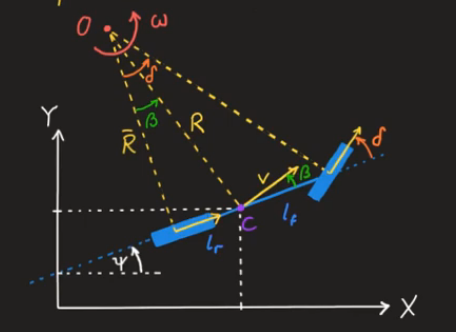
\includegraphics[width=0.8\linewidth]{bicycle_model.png}
        \caption{Bicycle model}
        \label{fig:bicycle_model}
    \end{figure}

    \subsubsection*{Pure Pursuit and Heading Error}
    Pure pursuit is a tracking algorithm that works by calculating the curvature that will move a vehicle
    from its current position to some goal position. The whole point of the algorithm is to choose a goal
    position that is some distance ahead of the vehicle on the path. The name pure pursuit comes from
    the analogy that we use to describe the method. We tend to think of the vehicle as chasing a point
    on the path some distance ahead of it - it is pursuing that moving point. That analogy is often used
    to compare this method to the way humans drive. We tend to look some distance in front of the car
    and head toward that spot. This lookahead distance changes as we drive to reflect the twist of the
    road and vision occlusions\cite{coulter1992implementation}.

    The heading error (HE) is the key parameter to be estimated, as it is the
    starting point of the pure pursuit control strategy\citep{7796574,9368694}.
    The HE is defined as the angle between the vehicle heading direction and the
    line that connects the lookahead point and the center of rear axle of the
    vehicle. The lookahead point is defined as the point on the path on a fixed (or
    variable) distance ahead of the vehicle. 
    \begin{align}
        \delta=\tan^{-1}\left(\frac{L\dot{\theta}}{v}\right)=\tan^{-1}\left(\frac{L}{R}\right)=\tan^{-1}\left(\frac{2L\sin\left(\alpha\right)}{l_{c}}\right)
    \end{align}

    The distance of the lookahead point
    is a delicate parameter, since a big value can lead to cutting curves at low
    speed and a too small value can lead to unstable behaviors at higher speeds.
    Moreover, the accuracy of the estimation is also affected by this distance,
    since it becomes more difficult to identify the lines which are far ahead.
    For these reasons an analysis on the lookahead distance is necessary. 

    In the practical implementation used to generate the training datasets in
    the simulator, we assume to have an \textit{optimal} path\footnote{The optimality of the path will be discussed in
    more detail in later sections.} that follows the center of the lane. The
    implementation follows the same approach explained in
    \citep*{coulter1992implementation}; in particular, the basic steps of the
    algorithm are:
    \begin{enumerate}
        \item Calculate the closest point $p_0$ on the path to the vehicle position,
        using the standard euclidean distance.
        \item Calculate the lookahead point on the path, using the lookahead
        distance $l_c$ from $p_0$. In this case we consider the arc
        length\footnote{The reasons behind the use of the arc length rather than
        the standard euclidean distance is that the existence and uniqueness of
        the lookahead point is guaranteed only by using the arc length.
        Moreover, for small curvature paths, the metrics lead to very similar values.}
        \item Convert the lookahead point to the vehicle coordinate system
        \item Calculate the heading error
    \end{enumerate}
    It is important to note that this process makes use of the position and
    orientation of the vehicle in the global frame of reference; therefore it
    can be used only in a simulated environment. This is indeed the algorithm
    used to generate the training datasets. 

    \begin{figure}
        \centering
        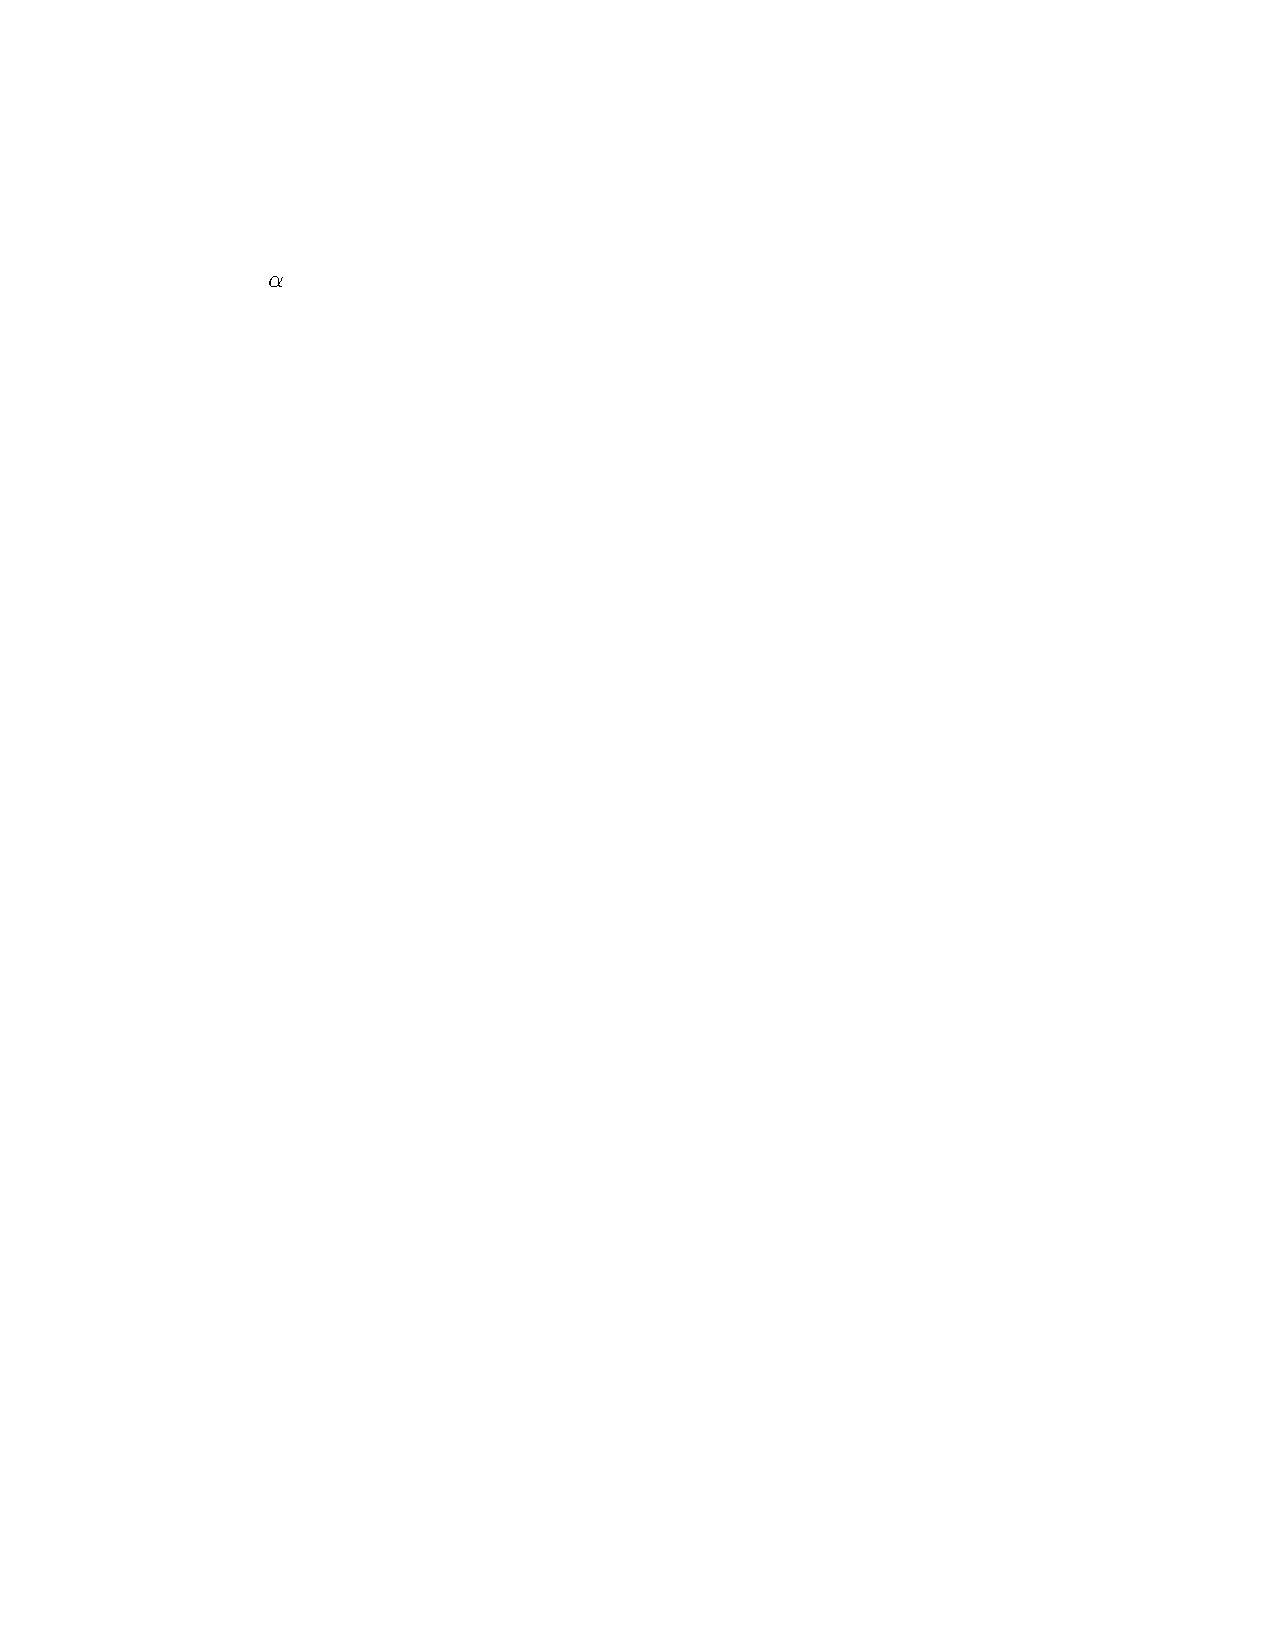
\includegraphics[width=0.6\linewidth]{a.pdf}
        \caption{Heading Error}
        \label{fig:heading_error}
    \end{figure}

    \subsubsection*{Camera}
    The camera is the main sensor used to perform the heading error estimation.
    In the model car it is positioned about 20 cm above the ground. It is oriented 20 degrees downward in order to see also the closer
    section of the road. The camera is a standard \textit{Raspberry Pi Camera}
    module. The technical specifications of the camera are the following:
    \begin{itemize}
        \item Still resolution: 8 Megapixels
        \item Video capture resolution: up to 1080p30, used at 640x480p at
        ~30fps (max 90fps)
        \item Focal length: 3.04 mm
        \item Horizontal field of view: 62.2 degrees
        \item Vertical field of view: 48.8 degrees
        \item F-stop: 2.0
    \end{itemize}
    The native resolution used is 640x480 since it allows for a better
    frame rate, however the images will be further reduced in size in order to
    increase performance. The simulated camera is mounted in the exact same
    position of the real one, and has been programmed to have the same field of
    view and frame rate.  

    \begin{figure}
        \centering
        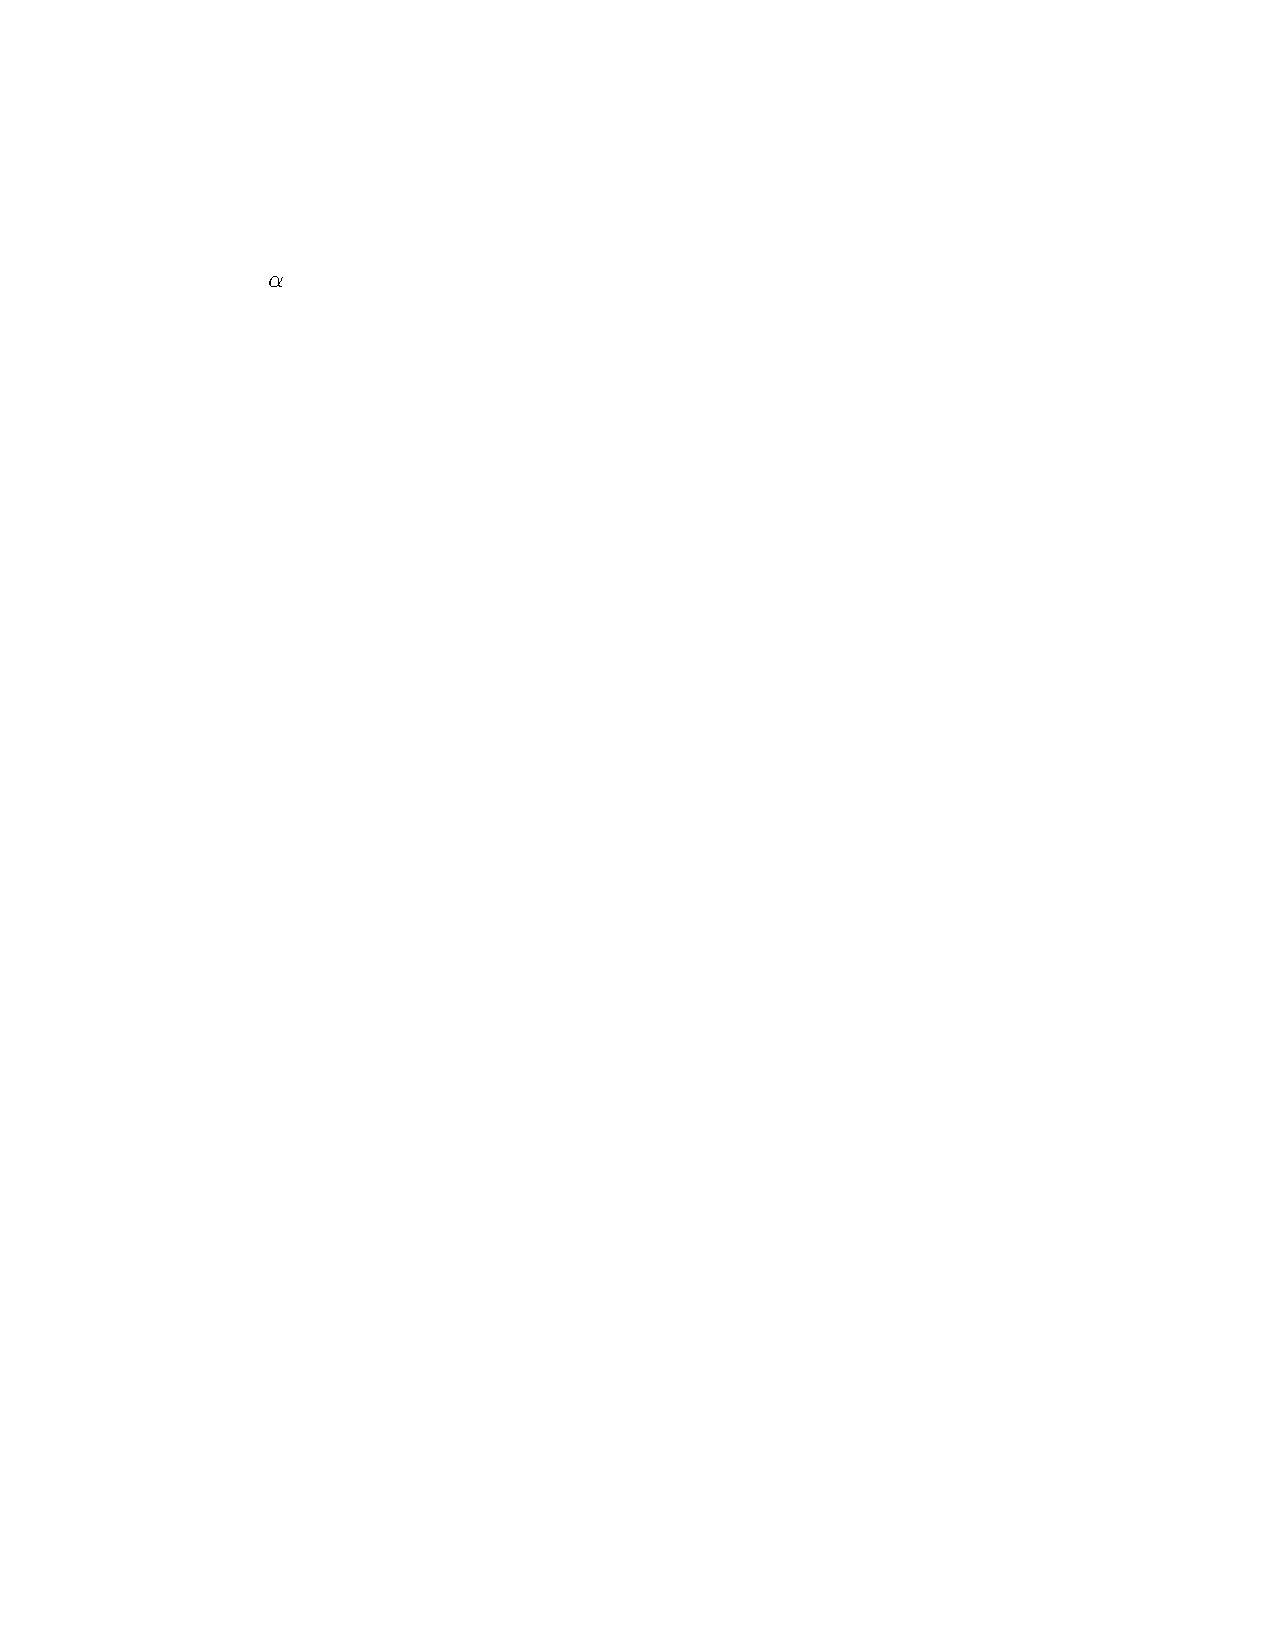
\includegraphics[width=0.6\linewidth]{a.pdf}
        \caption{Example image from the camera}
        \label{fig:camera_example}
    \end{figure}
    

    \subsection{Simulation environment}
    The simulation environment is a key component of the estimation process, it
    is not directly related to the online estimation itself, but it is used to
    generate the training datasets; the accuracy of the estimation is therefore
    extremely correlated with the quality of the dataset and, consequently, with
    the quality of the simulation. 

    For the simulation environment, we use the \textit{Gazebo
    simulator}\citep*{1389727}, which is a powerful simulator normally used in
    robotics. The reasons behind the use of this simulator are the fact that
    it's open source and does not require extreme hardware to run, moreover we
    were able to use assets that were given to us by the organizers of the
    challenge. In the following are listed the main characteristics of the
    simulation environment:
    \begin{itemize}
        \item It is a physics-based simulator
        \item The simulation is modular, allowing for the use of different
        models 
        \item \textit{Gazebo} is fully integrated with \textit{ROS}, this allows
        for easy access to all the sensors and actuators of the simulated
        vehicle and control of the simulation.
        \item The basic environment is composed of the model of the car and the
        streets, depending on the need it is possible to add other vehicles,
        pedestrians, and ramps.
        \item The car model is composed as a group of links/joints, with their
        respective physical properties. All the virtual sensors and actuators are
        mounted on the car model and are accessible through the \textit{ROS} network.
        \item The virtual camera is mounted in the exact same position of the
        real one, and it's configured to have the same field of view and frame
        rate. The flow of images is easily accessible through \textit{ROS}.
    \end{itemize}

    The simulator has been run on a laptop with an \textit{Intel Core i7-7500U}
    processor, an \textit{NVIDIA GeForce GTX 950M} graphics card and 16 GB of
    RAM.
    

    \begin{figure}
        \centering
        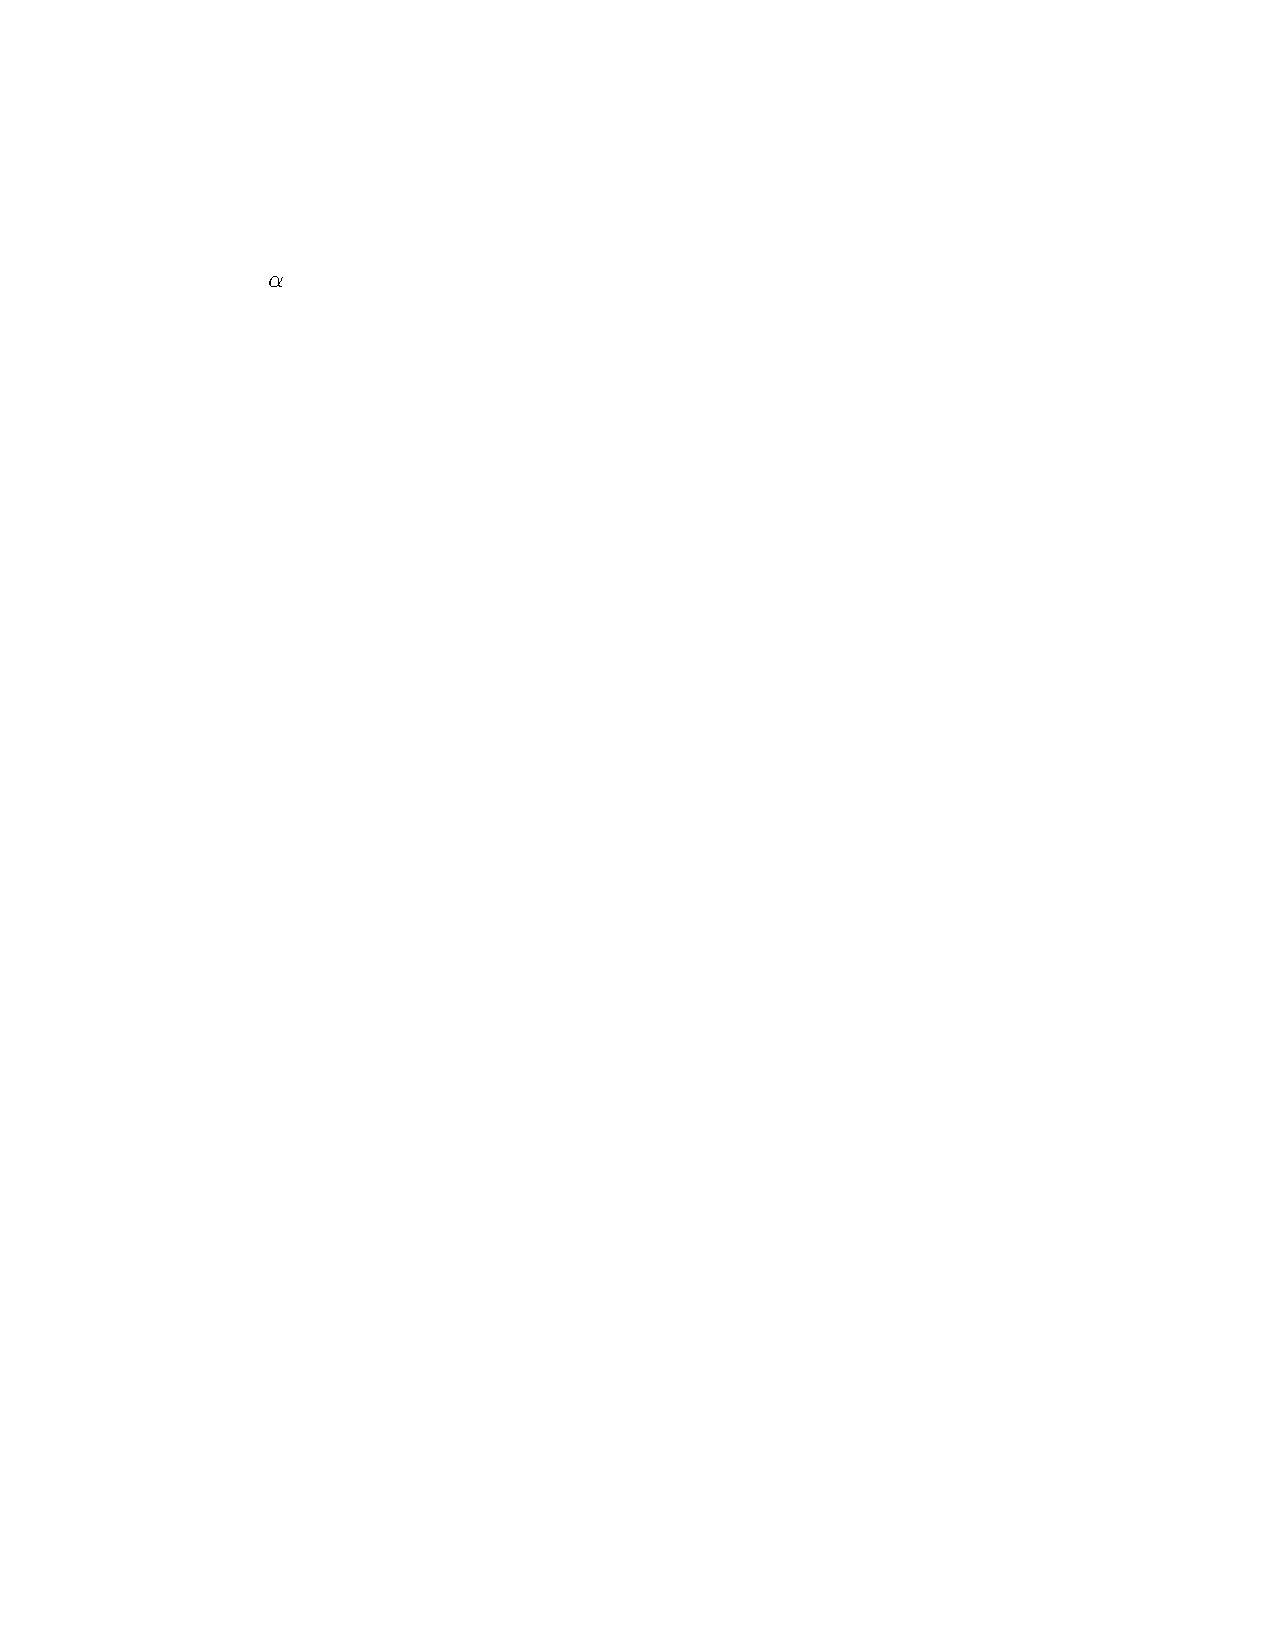
\includegraphics[width=0.6\linewidth]{a.pdf}
        \caption{ Simulator image }
        \label{fig:simulator}
    \end{figure}



\section{Optimal path}

    \subsection{Why do we need a path to follow?}
    The basic idea of having an \textit{optimal} path is being able to localize the vehicle on the
    path and to sample the heading error looking at the path ahead. 

    Since we are only interested in estimating the heading error with respect to the center of the
    road it does not seem necessary to have an optimal path; however there are several reasons
    why one would prefer a different path to the centerline. The first one is that the centerline
    could be an infeasible trajectory to follow for the vehicle, with an aggressive curvature or
    discontinuous first derivative. The second one is that the path
    method is very easy to scale in situations where the centerline is not clear or defined, for
    example when dealing with intersections or unmarked roads. The third is that it's possible to
    have some degrees of control over the path, for example on the smoothness or the maximum
    curvature. Moreover, the path concept is useful when planning far ahead in the future or when
    considering obstacle avoidance. Finally, using a path is very convenient from the implementation point of
    view, because it decouples the camera image from the localization and path tracking.

    \subsection{Why clothoids}
    Common path-planning methods usually generate obstacle-free path, but with no or very little concern
    about path feasibility or optimality so that it is usually necessary to apply some kind of transform
    algorithm to locally smooth such a path. Various path-smoothing algorithms are proposed in the
    literature: cubic splines \citep*{kanayama1988smooth}, intrinsic splines
    \citep*{delingette1991trajectory}, Bezier's curves \citep*{segovia1991comparative}, quintic
    Bezier splines \citep*{lau2009kinodynamic}, and clothoids. The main advantage of clothoids over
    other smoothing methods in path-planning
    applications is linear change of their curvature, which is of great importance for transportation of
    people or heavy and sensitive loads since it prevents abrupt changes in the centripetal acceleration
    and forces experienced by a vehicle increasing driving comfort. Clothoids are very attractive in
    path-smoothing applications as they are easy to follow because of their linearly changing
    curvature \citep*{shanmugavel2010co}. 

    Clothoids also have advantages over other smoothing techniques in sense of vehicles optimal motion
    planning—by applying the Maximum Principle from the optimal control theory, for forward
    motion and differential drive vehicle, one can find that the necessary condition for
    trajectory to be time optimal yields clothoids \citep*{388788}. Further, Boissonnat  et al.
    \citep*{BOISSONNAT1999613}  studied
    the shortest plane paths joining two given positions with given tangent angles and
    curvatures along which the tangent angle and the curvature are continuous and the derivative
    of the curvature is bounded. They showed that at a point where such a path is of class $\mathcal{C}^3 $,
    it must be locally a piece of a clothoid or a line segment. Similarly, Fraichard and Scheuer
    \citep{1362698} showed that with requirements of continuous curvature and bounded both curvature and its
    derivative, the shortest path consist of line segments, circular arcs, and clothoids \citep*{6646277}.

    \subsection{Clothoid definition}
    A Clothoid, also known as Euler or Cornu spiral, is a plane, invariant spiral curve defined in
    parameter form. As explained in \citep*{7962257} Its curvature $\kappa$ can be expressed as a linear function of its arc length
    $s$:
    \begin{equation} 
        \kappa (s)=\kappa _0 + \sigma s, \quad \kappa _0, \, \sigma \in \mathbb {R} 
    \end{equation}
    where $\sigma$ is the sharpness of the clothoid and $\kappa _0$ is the initial curvature at
    $s=0$. The tangent or winding angle $\theta$ with respect to its arc length is given as:
    \begin{equation} 
        \theta (s)=\theta _0+\kappa _0 s+\frac{\sigma s^2}{2}, \quad \theta _0, \, \kappa _0, \, \sigma \in \mathbb {R} 
    \end{equation}
    where $\theta _0$ is the initial tangent angle at $s=0$. Thus, a general clothoid can be
    expressed in paremetric form as in \citep*{nutbourne1972curvature}:
    \begin{equation} 
        \mathbf {F}(s) = 
        {\left(
            \begin{array}
                {c} x_0+\int _0^s \cos \left(\theta _0+\kappa _0 u +\frac{\sigma u^2}{2}\right) \, du \\ 
                y_0+\int _0^s \sin \left(\theta _0+\kappa _0 u +\frac{\sigma u^2}{2}\right) \, du \\ 
            \end{array}
        \right)} 
    \end{equation}
    Based on the above definition, it is possible to define the elementary clothoid segment $\mathbf
    {F}_{{\mathcal {E}}}(s)$ with $\sigma = \sigma _\mathcal{E} > 0$, $s \geq 0$, $\kappa _0 \geq
    0$, $\theta _0 = 0$, $(x_0, y_0) = (0,0)$ and $\theta \in (0, \pi/2]$
    \begin{equation} 
        \mathbf {F}_{{\mathcal {E}}}(s)= \sqrt{\frac{\pi }{\sigma _{{\mathcal {E}}}}} \mathbf {R} 
        \left(
            -\frac{\kappa _{0}^2}{2 \sigma _{{\mathcal {E}}}}
        \right) 
        {\left(
            \begin{array}
                {c}\delta _c(s) \\ \delta _s(s)\\ 
            \end{array}
        \right)} 
    \end{equation}
    where $\delta _c(s) = C_f (\frac{\sigma _{{\mathcal {E}}}s+\kappa_0}{\sqrt{\pi \sigma
    _{{\mathcal {E}}}}}) - C_f (\frac{\kappa_0}{\sqrt{\pi \sigma _{{\mathcal {E}}}}})$ and
    $\delta_s(s) = S_f (\frac{\sigma _{{\mathcal {E}}}s+\kappa_0}{\sqrt{\pi \sigma
    _{{\mathcal {E}}}}}) - S_f (\frac{\kappa_0}{\sqrt{\pi \sigma _{{\mathcal {E}}}}})$. Here,
    $\mathbf {R}(\theta)$ is the standard planar rotation matrix, and $C_f(x)$ and $S_f(x)$ are a
    pair of nonnegative functions named Fresnel integrals \citep*{41470}:
    \begin{equation} \label{eq:clothoid}
        C_f(s)=\int _0^s \cos 
        \left(
            \frac{\pi \xi ^2}{2}
        \right) 
        \, 
        d\xi, \, S_f(s)=\int _0^s \sin 
        \left(
            \frac{\pi \xi ^2}{2}
        \right) 
        \, 
        d\xi . 
    \end{equation}

    \subsection{Implementation}

    The context of our particular application is the following: we are given a map of a scaled city,
    with roads, intersections, roundabouts, crosswalks, etc... Alongside with the map we are also given
    a set of waypoints in the form of a directed graph. Every waypoint corresponds to an $(x,y)$ position on
    the map, more specifically to point in the center of a lane. All the waypoints are placed at
    about $30 cm$ from each other. Every waypoint also incorporate a list of edges that
    connects it to other waypoints, in such a way that only consecutive waypoints are connected by an
    edge and only if they follow they same lane, the only exceptions being the points associated to
    roundabouts and intersections as well as the start point and the end point. 
    
    The goal of the algorithm is to take 2 waypoints as input and return a path that connects them.
    To achieve this goal, we start by finding the shortest path in the graph of waypoints that
    connects them\footnote{We restrict ourselves to the case where at least one path exists between
    any two waypoints, which was always true in our scenario, except if we considered the end point as
    starting point}; to do this we use the Dijkstra algorithm \citep*{dijkstra1959note}. 
    
    The second and last step to create the \textit{optimal} path is to fit clothoid segments between the
    waypoints of the shortest path. Since the Fresnel integrals in equation (\ref*{eq:clothoid}) are two transcendental functions,
    they can't be solved analytically, however there are several approximation
    methods in the literature that achieves good results \citep*{6646277,7962257,4543548}. In our
    implementation we used the python library \textit{pyclothoids} \citep*{pyclothoids}, which is a python
    wrapper of the C++ library by Bertolazzi \citep*{https://doi.org/10.1002/mma.3114, BERTOLAZZI201899,
    https://doi.org/10.1002/mma.4700, doi:10.1137/18M1200439}. 
    In figure \ref{fig:path} it is possible to see the result of the algorithm, the path is designed
    to cross most of the waypoints.

    \begin{figure}[h!]
        \centering
        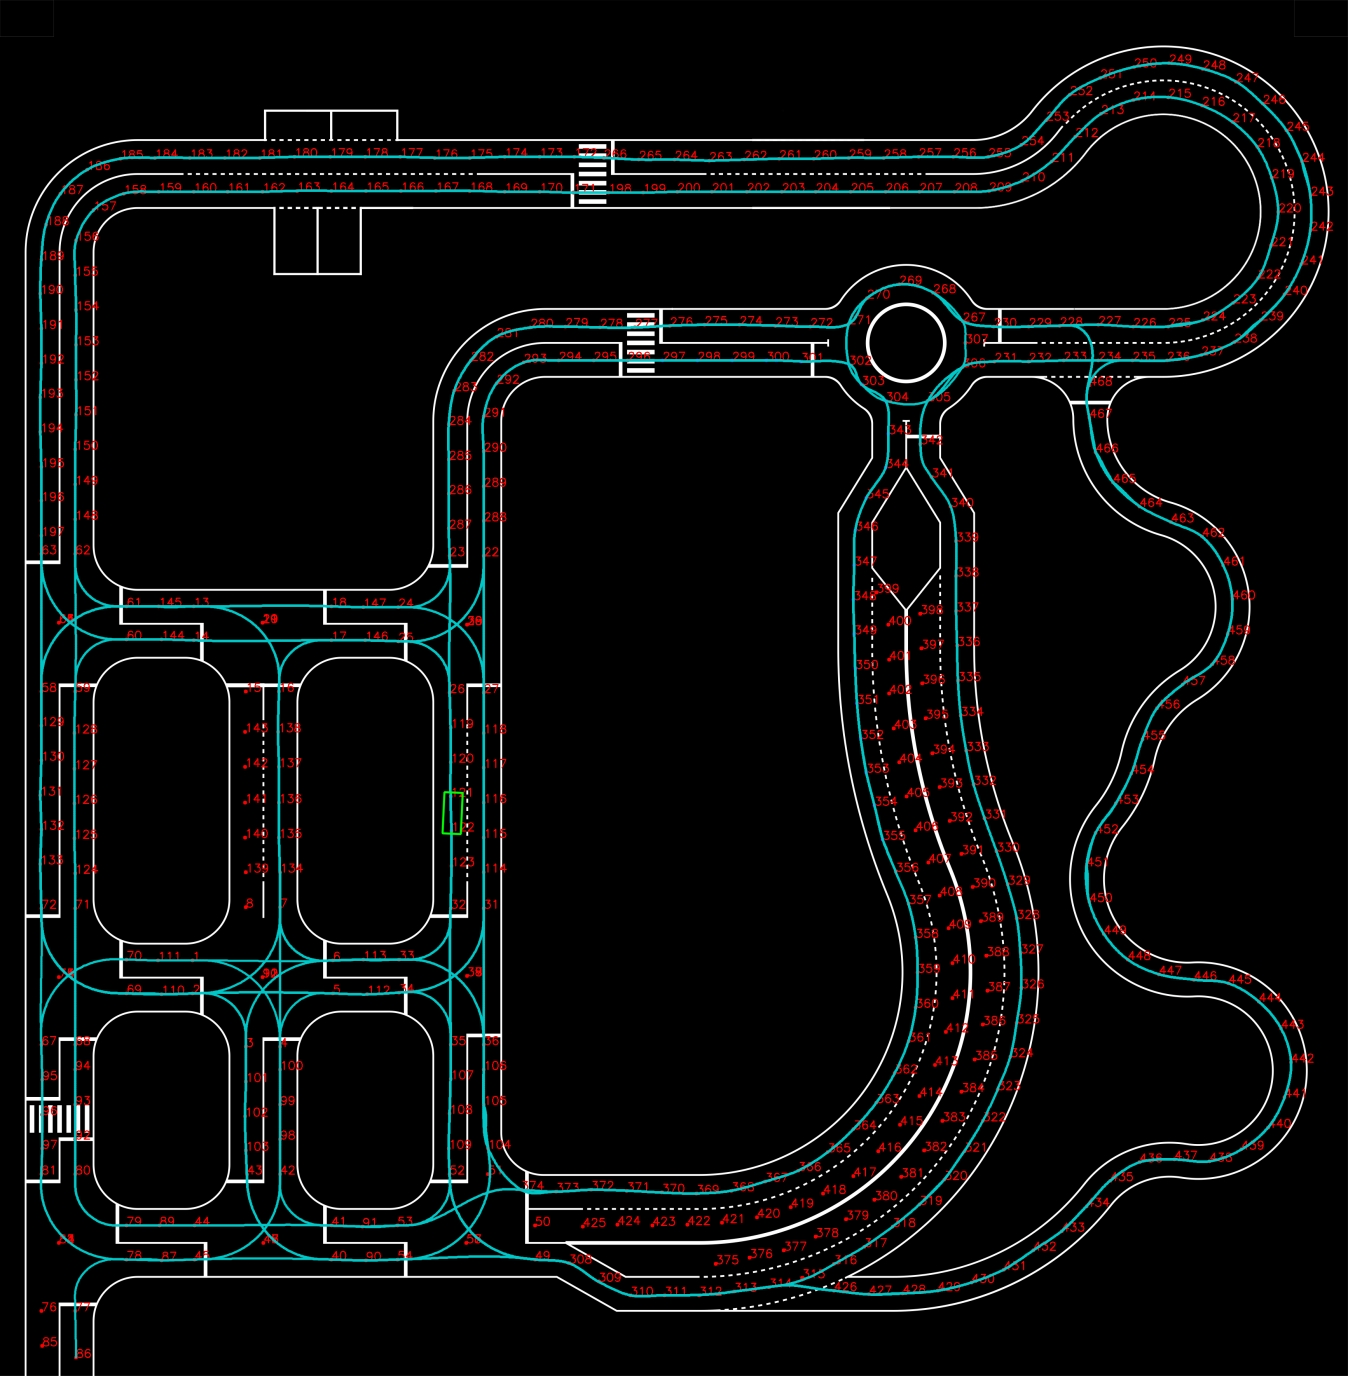
\includegraphics[width=\linewidth]{full_path.jpg}
        \caption{Map and waypoints, with the optimal path passing through most of the waypoints}
        \label{fig:path}
    \end{figure}


\section{Performance metrics}

    Since we are dealing with a complex estimation problem, it is very important to define a set of
    appropriate performance metrics in order to reliably evaluate the quality of the estimation.
    This is a difficult task since the problem of the estimate of the heading error with respect to
    the center line is strictly related to the problem of the road estimation itself. 

    In this section we will analyze a set of metrics found in the literature, and we will propose a
    different metric that we believe is more appropriate for our problem. 

    It is very important to make an initial distinction between two, very related but
    different, approaches to the performance evaluation of lane detection and tracking systems: the
    first one consists in comparing the estimation capabilities of the whole systems (estimation
    \textit{and} control) by means of evaluating the tracking performance in a real or simulated
    scenario. The second one consists in evaluating only the estimation performance on some kind of
    ground truth data. The first approach is more realistic, but it has some big drawbacks: it is
    very difficult to perform a fair comparison between different systems because it is hard to
    replicate the same conditions in every test; moreover a systematic analysis of a big parameter
    space with many possible variations is often infeasible within the testing time constraints.
    Lastly, a very important issue is that testing tracking performance in a real scenario doesn't
    give an accurate picture in terms of disturbances, or in other words, in situations where car is
    relatively far from the center line, or in some very rare or extreme configurations, since a
    good tracking systems is always close to tracking target in terms of both position and orientation. 
    The second approach is more specific to the estimation problem, and therefore less applicable to
    a wide range of systems. However, it has the advantage of being performed offline on prerecorded
    videos, guaranteeing a fair comparison between variations, and it is also possible to perform
    systematic sweeps over the parameters space in order to find the best configuration. In addition
    to this it's possible to evaluate performance on edge cases in a fair and systematic way.  For these
    reasons in this thesis we will focus on this second approach, analyzing the whole tracking
    performance as a final step.

    \subsection{Metrics from the literature}

    In the paper \citep*{6977166} we can see that in the analyzed methods, to evaluate performance,
    visual inspection of lane estimation is deployed in all studies. However, this is only a
    qualitative metric. In order to quantify the performance of a lane estimation technique, one of
    the most common metric is ego-vehicle position localization within the lane \citep*{1603550,cheng2007lane,6728507}.
    Lower error in ego-vehicle localization is a result of more accurate lane detection process
    itself. This is because ego-vehicle localization is computed using the estimated lane positions
    in the proximity of the ego-vehicle. The method we propose will be strictly related to this
    concept. Another key metric proposed in \citep*{6977166}, which is not very common in the
    previous literature, but very important for the implementation side of the problem, is the
    computational efficiency of the algorithm. Since we are dealing with a real-time problem, and
    relatively low computational power, this metric is very important in our application.

    Other, more quantitative, proposed metrics are the following:
    \begin{itemize}
        \item Lane markings related metrics: this set of metrics, despite being useful in some
        applications, has been discarded since the estimation target doesn't directly depend on the
        markings themselves, and could potentially be used in a scenario where there are no
        markings at all, or very non-standard ones. In addition to this, one should consider the
        additional complexity, and the appropriate way of generating the estimate of the lane
        markings, which is not a trivial task and not the object of this thesis.
        \item Pixel level accuracy: this metric is very widely applied in the context of vision
        based estimation, it consists in classifying each pixel of the image as either part of the
        lane or not. It is a very common in deep learning approaches \citep*{9398517}, firstly because it's very
        straightforward to implement using convolutional filters and secondly because most of the
        training and evaluation datasets are annotated pixel by pixel. This metric is usually
        evaluated by means of a ratio between the number of correctly classified pixels and the
        total number of pixels. This metric is not very useful in our case, since we are
        interested in the heading error, however it is a very interesting possible extension of the
        proposed method.
    \end{itemize}
    There are several other metrics in the literature that are of little interest in our particular
    application. 

    \subsection{Proposed metric}
    Since in our particular application we are interested in the heading error, which is a scalar
    quantity, a very natural choice for a performance metric is the mean squared error (MSE) with
    respect to the ground truth. The main issue with this approach is how to retrieve the ground
    truth. In the simulated environment it is very easy since we have access to the precise absolute position
    and orientation of the car. In the real case it is more challenging, but with the experimental
    setup we used, explained in section \ref*{sec:exp_setup} we were able to retrieve a precise
    position and orientation, therefore we have an accurate ground truth that can be used to
    evaluate the estimation performance and to compare different methods. In addition to the MSE,
    the mean absolute error can also be considered with the same rationale, which is less dependent
    on outliers. 

    Another considered metric is the continuity and smoothness of the output sequence,
    meaning that a sequence of consecutive frames should generate a continuous smooth output sequence
    of heading errors, since we are not expecting any sudden changes in the road ahead or in the car
    position. This metric becomes particularly important if we plan to use a control system on top
    with some parameters that are dependent on the variation of the heading error, like, for
    example, a PID controller with a derivative term. 

    Lastly, we can also consider the computational efficiency of the algorithm and the
    generalization capabilities of the system from the simulated environment to the real one, which
    is a very important aspect of this estimation method.  

    \begin{figure}
        \centering
        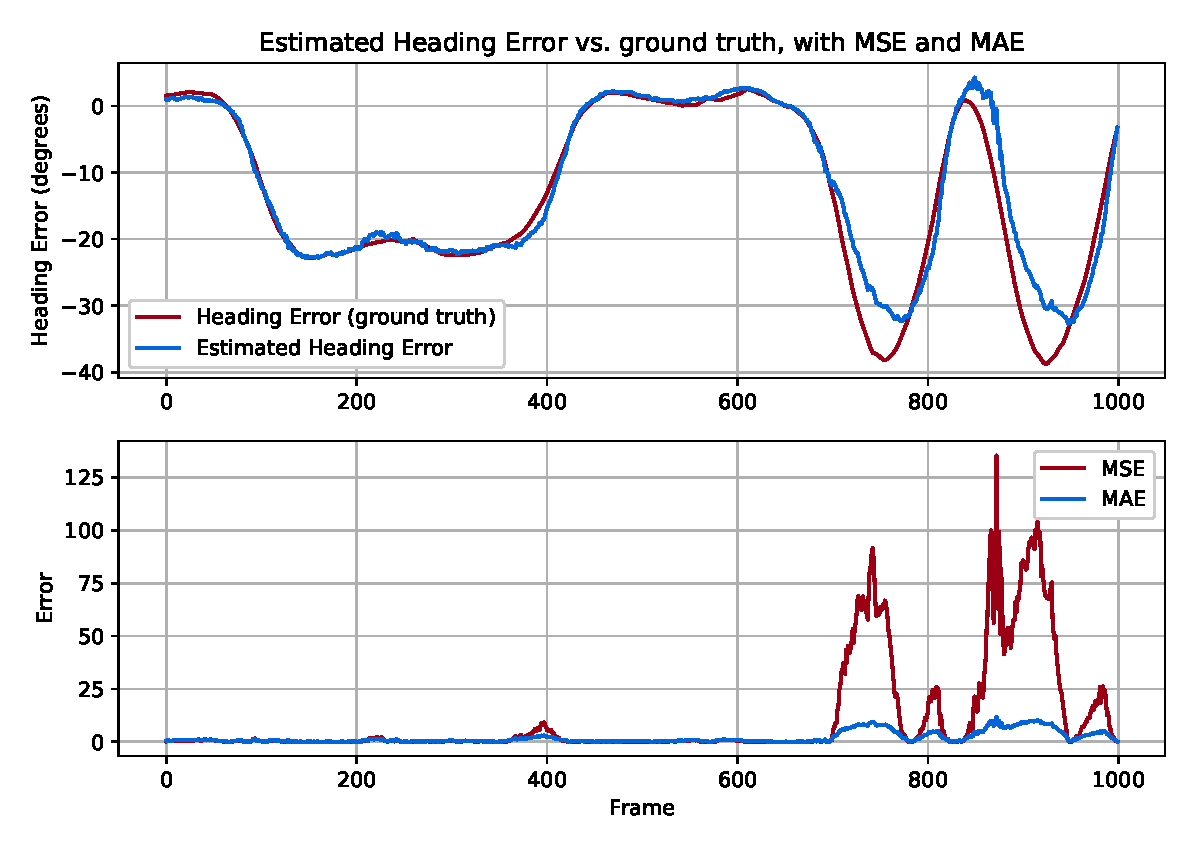
\includegraphics[width=\linewidth]{figures/performance_metrics_example.eps}
        \caption{Performance metrics example}
        \label{fig:performance_metrics_example}
    \end{figure}


    % Definizione delle metriche di  performance s

    % Read code not pdf here...
    % -L2 norm that we have both in simulation and hopefully in the real world thanks to a precise
    % localization system (my idea)
    % -The ones explained in 'On Performance Evaluation Metrics for Lane Estimation'
    % \url{https://ieeexplore.ieee.org/abstract/document/6977166}
    %     -there are several citated
    %     -some are qualitative
    %     -some evaluate the whole system estimation+Controller
    %     -accuracy of lane markings wrt ground truth
    %     -variance of polynomial coefficients that define lanes
    % -The ones explained in section 5 of 'Video-based lane estimation and tracking for driver
    % assistance: survey, system, and evaluation' \url{https://ieeexplore.ieee.org/document/1603550}
    %     -they used mean absolute error in position, standard deviation of error in position, standard
    %     deviation of error in rate of change of lateral position
    %         the idea of the rate of change is very interesting
    %     -they also cite \url{https://ieeexplore.ieee.org/document/660563}, which are the
    %     angular-deviation entropy and angular-deviation histogram fraction and their magnitude-weighted
    %     counterparts. 
    % -We should consider the 2 cases: the case of the heading error estimation and the case of the
    % actual lane detection, there should be 2 different performance metrics for each one of them
    % -We should consider the fact that we have the simulation environment and evaluate the performance
    % in easy conditions, namely when the tracking is near the center of the road, or when the car is
    % sliding left and right
    % -we should evaluate the continuity of the output as a performance measurement
    % -also we should distinguish the performance metric of the road estimation, from the whole
    % estimation+tracking performance, in this paper we are interested only in the first one. 
    % -check papers: \url{https://ieeexplore.ieee.org/document/6728473},
    % \url{https://ieeexplore.ieee.org/document/9398517}, which are more about the deep learning
    % aspect
    %     -pixel level correctness (intersection over union) with evaluation on predef datasets
    %     -boundary position and deviation
    %     -corridor width

    % -computational efficiency
    % -different performance metrics for different sections (curves, straight lines)
    
    % -CONTINUITY
    % -RMS SU HE E DERIVATA

    % useful papers:
    % \url{https://ieeexplore.ieee.org/abstract/document/6977166, https://link.springer.com/article/10.1007/s00138-011-0404-2, https://ieeexplore.ieee.org/document/1603550, https://ieeexplore.ieee.org/document/6728473,  https://ieeexplore.ieee.org/document/9398517} 


\newpage

\section{Proposed estimation method}
In this section we will present the proposed method for the estimation of the heading error. From a
general point of view the process can be subdivided in 5 main steps that will be described in detail
in the following subsections:
\begin{enumerate}
    \item \textbf{Data collection}: this step consists in collecting, in the simulated environment,
    the raw data that will be used to generate the datasets.
    \item \textbf{Heading error calculation}: the second step is to generate the ground truth for the
    previously generated datasets. It's important to separate this step from the previous one, in
    order to allow a more general approach to the problem.
    \item \textbf{Dataset generation}: this step consists in generating the datasets that will be used to
    train the network, it is when data preprocessing and augmentation are applied, 2 key components
    of the proposed method.
    \item \textbf{Network training}: this step consists in training the network using the previously
    generated dataset. The network architecture will be discussed, together with the training
    process itself and the hyperparameters used. 
    \item \textbf{Online estimation}: this is the final step, where all the previous steps are combined in
    order to accurately estimate the heading error in real time, on the real vehicle, from the
    camera frames.
\end{enumerate}

\subsection{Data collection}

The main idea of data collection is to use the \textit{Gazebo} simulator to generate an arbitrarily
large set of images and the corresponding ground truth labels. During the developing process 2 main
methods were designed in order to solve the task. The original method was tailored to the specific
aspects of the challenge, and was therefore designed to solve not only the data collection problem
but also any other aspect of the challenge that could be tested in a simulated environment, such as
the high level logic, the control system, the interface with the additional simulated sensors, etc.
The second method was designed after the challenge to be specific with respect to the data
collection problem. The second method heavily simplifies the interface and the complexity required
to control the car in the simulator, and allows to generate the dataset with a much finer level of
control. In order to study the influence of the dataset collection parameters on the final
performance, in this thesis we will use and focus mostly on the second method, however the original
method will also be described since it shares most of the ideas.

\subsubsection*{Original method}
The Gazebo simulator is very convenient for developing since every simulated model and sensor
information is published on a \textit{ROS} topic, and the car can also be controlled by publishing
steering and throttle commands on their respective topics. This is very useful since it allows to
use the same code for both the simulation and the real vehicle, where we also implemented a
\textit{ROS} network. 

The main steps of the original method are the following:
\begin{itemize}
    \item A training path is generated for the car to follow, this path is based on the
    aforementioned Clothoid interpolation and slides across all the different sections of the map in
    order to allow the car to encounter a good variety of situations.
    \item The car is controlled with a PP controller at a fixed speed. 
    \item The point ahead for the controller is selected by finding the closest point of the vehicle
    on the path and then choosing the point on the path at a fixed distance ahead of it. This way of
    selecting the point ahead is very convenient and easy to implement and has the advantage of
    always finding a unique point, but is not conformed to the common definition of point ahead for
    the PP controller. 
    \item While the vehicle is travelling along the path, Gaussian noise is injected into the
    steering in order for the car to slide left and right. This is done in order to generate more
    variety in the training dataset. The noise injection is a key aspect of the estimation method
    and has a big impact on the final performance, as it will be discussed in section
    \ref*{sec:results}. The idea is that if the camera only sees the road ahead always perfectly
    centered, later, after the training, when facing the road at a different position and
    orientation, slightly off center, the network will not be able to estimate the heading error for
    lack of examples in the training dataset. The amount and characterization of the noise injected
    will be subject of a parametric analysis.
    \item While the car is travelling, the camera is recording images at a fixed rate of 30 fps and
    saving them alongside their corresponding ground truth heading error in a compressed file for
    later use. 
\end{itemize}
The 2 main advantages of this method are the flexibility and the wide variety of possible scenarios.
The main disadvantages are the complexity of the implementation, the lack of precise control over
the noise injected and the fact that the heading error distance is fixed and cannot be changed after
the dataset has been generated.

\subsubsection*{New method}
The new data collection method is designed to solve the previous method main issues: reducing the
code complexity, fine controlling the noise injected and generate the heading error independently of
the images. To achieve this, we apported a series of modifications:
\begin{itemize}
    \item The entire interface with the simulated car is removed, the vehicle is moved around the
    simulated environment by teleporting it to the new desired position an orientation using a
    \textit{ROS} service. In this way we are able to directly control the variance of the noise both
    in the car orientation and lateral position with respect to the lane center by sampling from 2
    Gaussian distributions; the change effect can be seen in image \ref*{fig:original_vs_old}. In
    this way we don't  need a controller anymore.
    \item The map and the path are simplified to a single loop designed to match the real track we
    built in the university's laboratory for the real-life tests. This allows to isolate only the
    lane detection problem, and it's a practical test bed for performing systematic tests and
    evaluate their performance. 
    \item To disconnect the heading error calculation from the image generation, the images are
    saved alongside the respective car position and orientation, and the heading error can be
    calculated offline for any distance using the more accurate method described in the following
    section.   
\end{itemize}


\begin{figure}
    \centering
    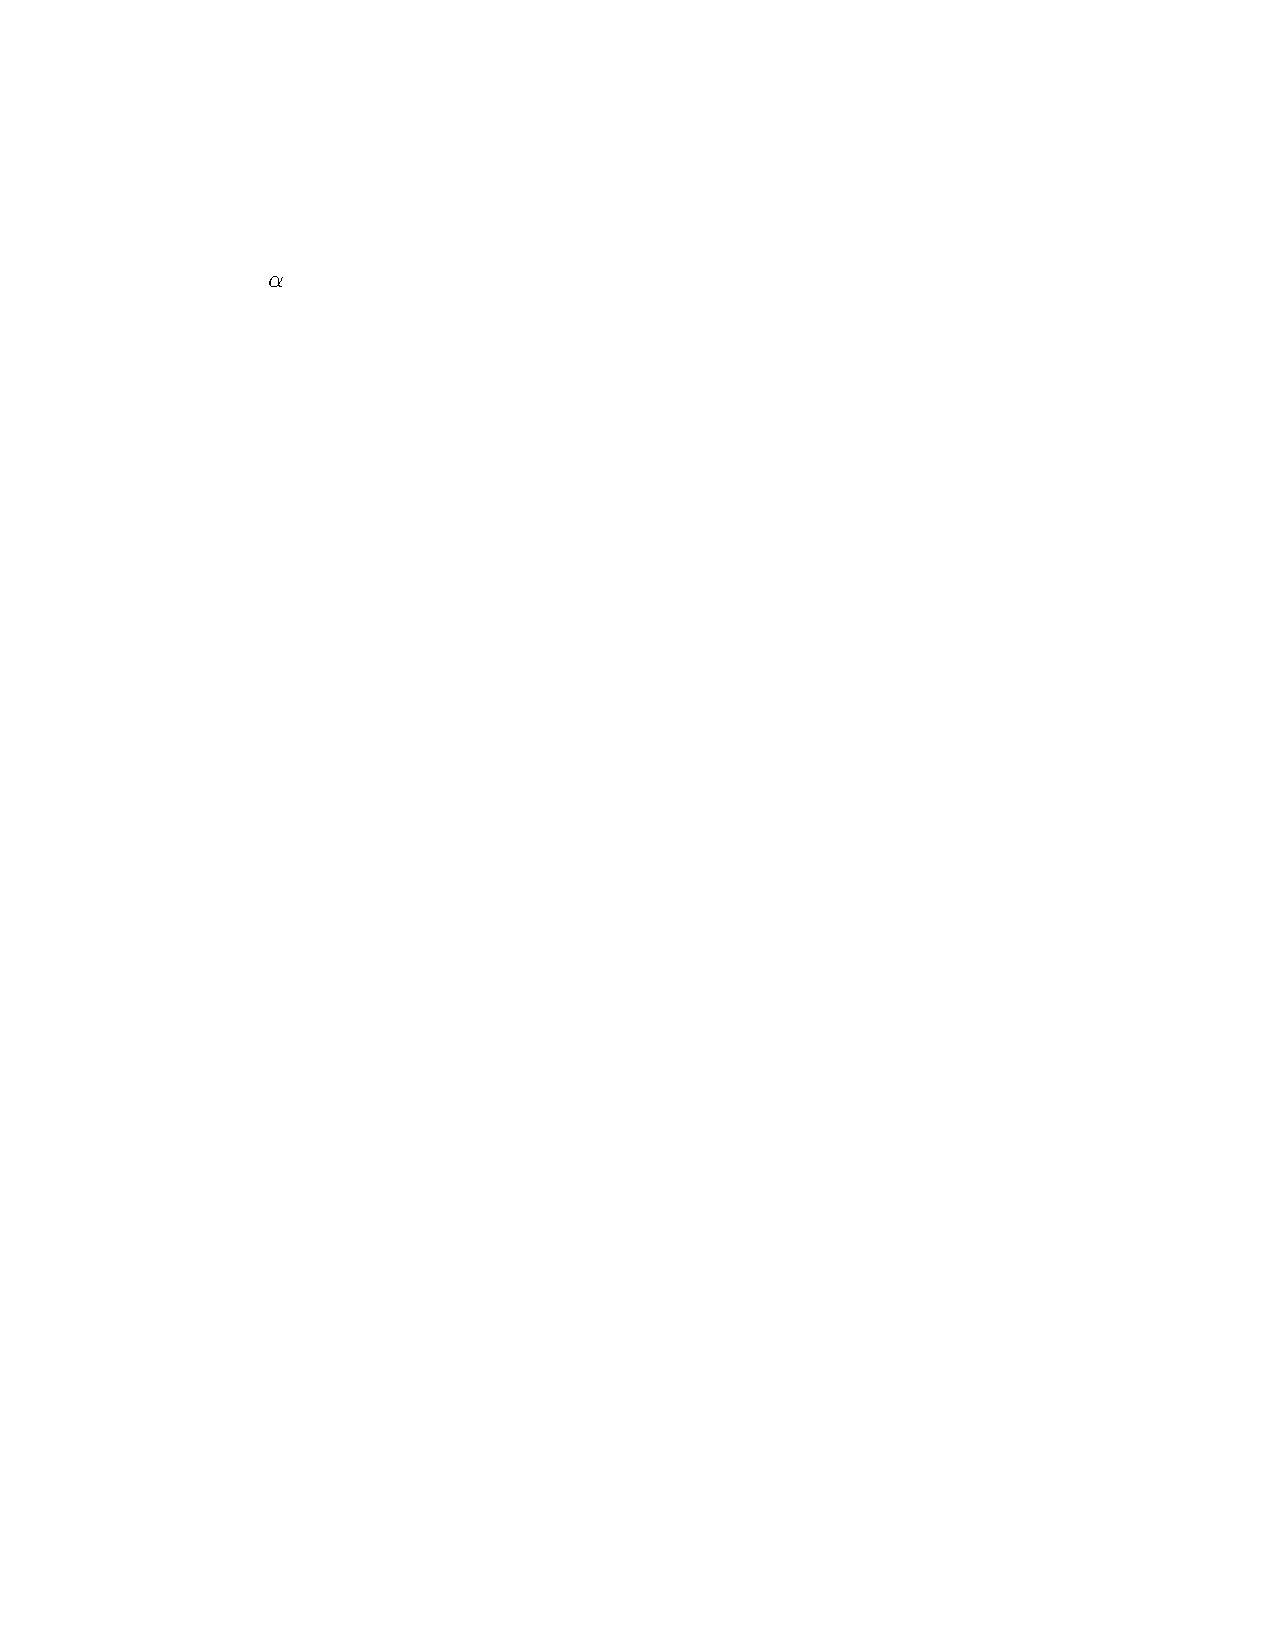
\includegraphics[width=0.6\linewidth]{a.pdf}
    \caption{Original method and new method}
    \label{fig:original_vs_old}
\end{figure}

%explain the main steps of the pipeline
% -Data collection
% -explaining data collection in simulator
% -how all the pieces come together
% -reasons behind the choices
% -(explaining data collection in real world, better explained in results sections)
%     -dependency on possible parameters:
%     -noise level in steering, can be evaluated both a priori(type of noise injection) and a
%     posteriori(variance between optimal path and training path), 
%         -noise level in speed
%         -number of frames
%         -fps of the Video
%         -length of Video
%         -length of simulation path
%         -(variability of the path, choosing a very repetitive path or a variable one)
%         -(camera orientation, requires redoing all videos)
%         -(camera position, requires redoing all videos)

\subsubsection*{Heading error calculation}
    In order to precisely calculate the heading error an algorithm has been developed that is a
    direct implementation of the common heading error definition in the PP controller
    \citep*{9368694}. The algorithm works by first finding the (normally 2) points at the distance
    $d_ahead$ required, and then selecting the one that is coherent with the car orientation. The
    algorithm is robust with respect to the 2 possible edge cases of finding a single point or no
    point at all, which means the vehicle is too far from the path and the algorithm returns the
    closest point; or the one where there are $\geq 2$ points at the same distance, in this case the
    algorithm returns the further in the path. The algorithm is implemented in python and a
    pseudocode for it can be seen in Algorithm \ref*{alg:heading_error_calculation}. A graphical
    intuition of the algorithm can be seen in figure \ref*{fig:heading_error_calculation}. 
    
    \begin{algorithm}
        \caption{Calculate Heading Error}\label{alg:heading_error_calculation}
        \begin{algorithmic}[1]
        \Procedure{$\text{calcHE}, \text{inputs}: x,y,\phi, path,d_{ahead}$}{}
        \State $thrsh \gets \text{ distance between points in } path$
        \State $p_{car} \gets \text{create point } (x,y)$    
        \State $p_0 \gets \text{projection of } p_{car} \text{ on } path$
        \State $\text{roll } path \text{ to make } p_0 \text{ first}$
        \State $path_a,path_b \gets \text{ split } path \text{ in half}$ 
        \State $D_a \gets | \lVert path_a - p_{car} \rVert - d_{ahead}| \text{  }$  \#vector of
        distances ahead
        \State $D_b \gets | \lVert path_b - p_{car} \rVert - d_{ahead}| \text{  }$  \#vector of
        distances behind
        \State $i_a \gets \text{argmin } D_a,\text{ } i_b \gets \text{argmin } D_b$   
        \State $min_a \gets D_a[i_a], min_b \gets D_b[i_b] \text{ }$ \#minimum distances
        \If {$min_a \geq thrs \textbf{ or } min_b \geq thrs$ \text{ }} \#car too far from path
        \State $p_{HE} \gets p_0$
        \Else $\text{ }$\#select the further point
        \State $p_a \gets path_a[\text{max}(\text{where}(D_a < thrsh))] \text{ }$ 
        \State $p_b \gets path_b[\text{min}(\text{where}(D_b < thrsh))] \text{ }$
        \State $p_p \gets p_{car} + d_{ahead}(\text{cos}\phi, \text{sin}\phi)\text{ }$ \#project car
        heading
        \State $p_{HE} \gets \text{ closest point to } p_p \text{ between } p_a \text{ and } p_b$
        \EndIf
        \State $\phi_{ref} \gets \text{atan2}(p_{HE}[y] - p_{car}[y], p_{HE}[x] - p_{car}[x])$
        \State \Return $\phi_{ref} - \phi$
        \EndProcedure
        \end{algorithmic}
    \end{algorithm}

    \begin{figure}
        \centering
        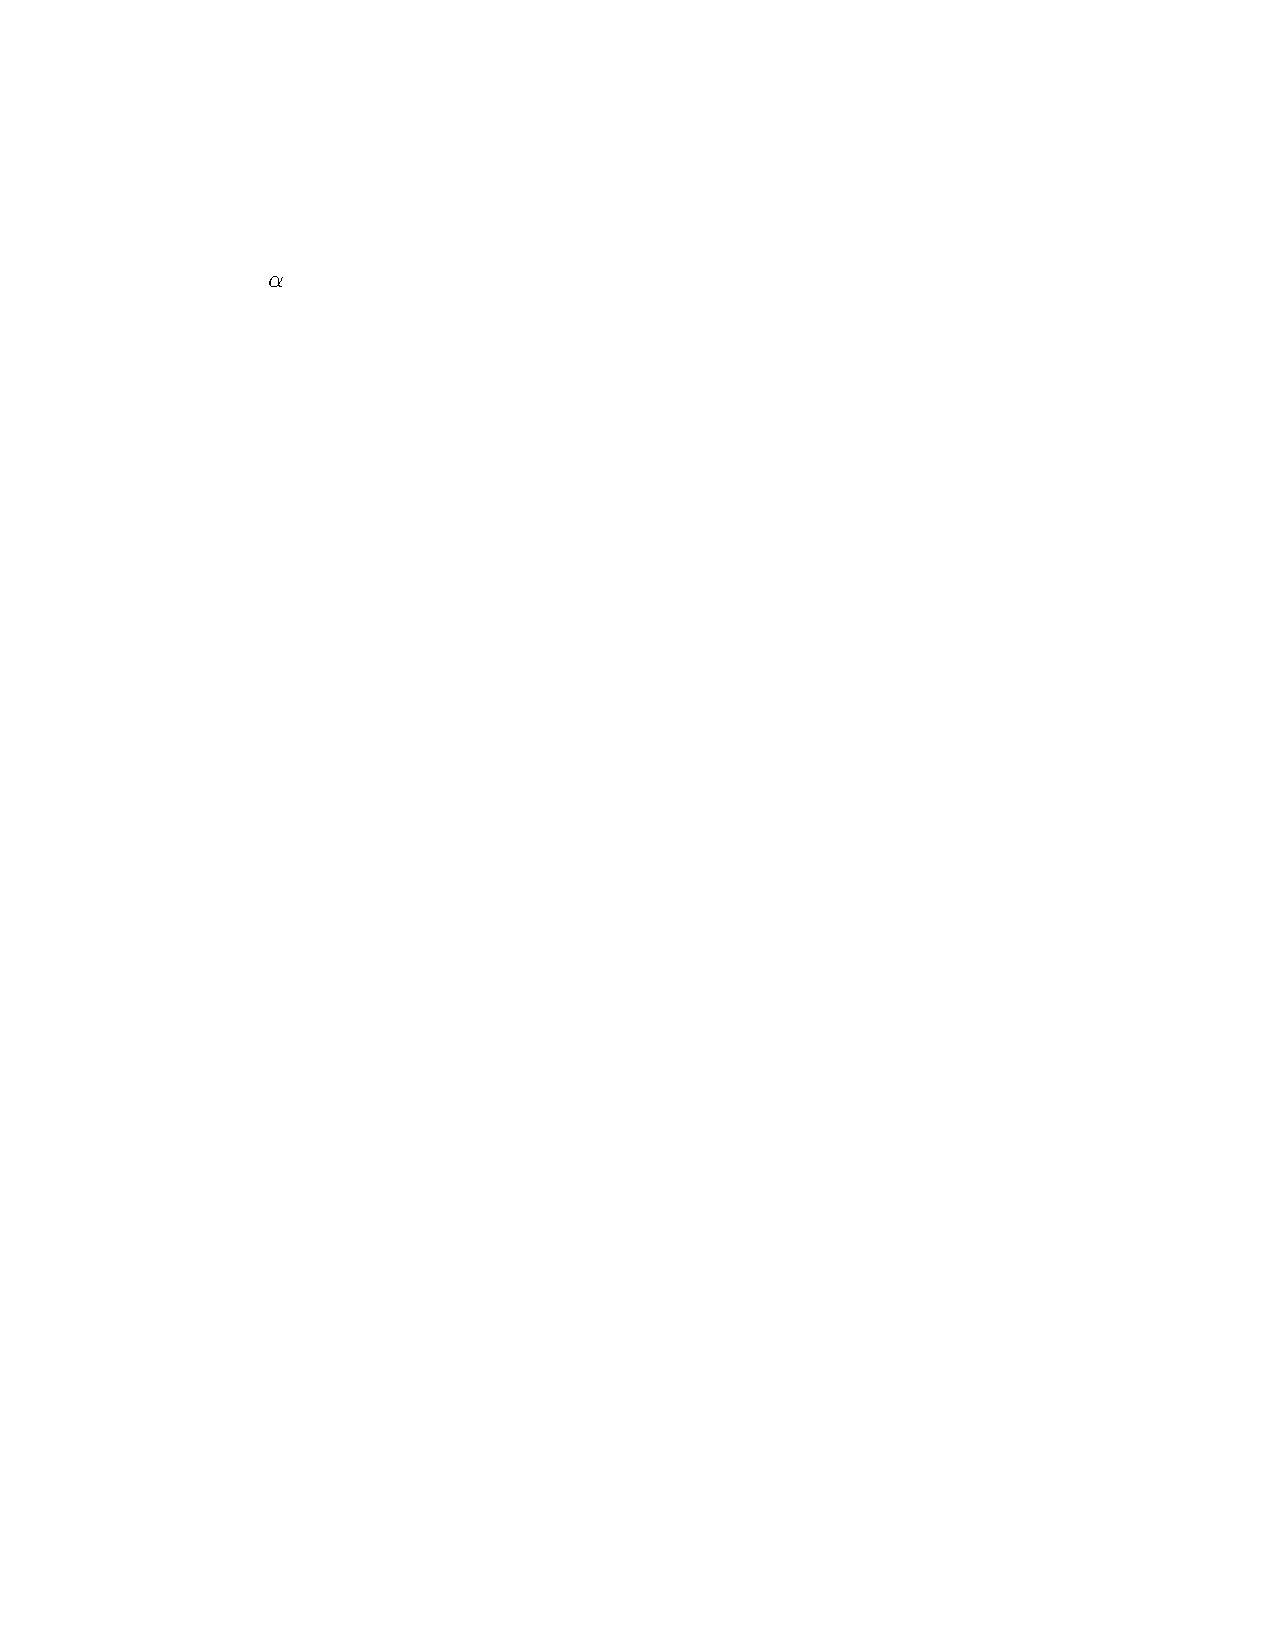
\includegraphics[width=0.6\linewidth]{a.pdf}
        \caption{Heading error calculation}
        \label{fig:heading_error_calculation}
    \end{figure}


\subsection{Dataset generation}
    With dataset generation we mean the process of converting the collected raw data into
    well-defined dataset that can be used for training. In this section we will discuss the 2 main
    steps for the images to be ready for training: image preprocessing and image augmentation.

    \subsubsection*{Image preprocessing}
    Image preprocessing is applied both to the images collected in the simulator and to the images
    processed in real time for online estimation. The 3 main goals of the preprocessing are reducing the 
    amount of information in the image to the minimum required for the task at hand, standardizing
    the images to make the real and simulated data more comparable, and reducing the computational 
    cost. The preprocessing main steps are the following:
    \begin{itemize}
        \item \textbf{Gray scale conversion}: all the images are converted from RGB to gray scale.
        This is done because the color information is not relevant for the task at hand (and the
        images are already mostly black and white) and because it reduces the computational cost.
        \item \textbf{Crop}: the images are cropped to remove the top section. The reason for this
        is the fact that the top section of the image contains the sky and the horizon and the very
        far away section of the road, which does not contain any relevant information. The
        percentage of the image kept is a hyperparameter that can be tuned. The influence of this
        parameter will be discussed in the Results section (\ref*{sec:results}).
        \item \textbf{First resize}: the images are resized to double the final size. In this case
        to a square of 64x64 pixels. This is done to reduce the computational cost of the algorithm
        and to preserve only the most predominant features of the image. The reason for the square
        is that is very convenient for the convolutional neural network to have the same number of 
        pixels in the height and width of the image.
        \item \textbf{Canny edge detection}: the images are processed with the Canny edge detector
        \citep*{canny}, which is a very common edge detection algorithm. Edge detection is the key
        component for making the images more comparable between the real and simulated data, since
        it removes any brightness and contrast variations that are present in the real images, and
        outputs a binary image. The Canny algorithm has 2 parameters that can be tuned to filter the
        edges by strength and by length.   
        \item \textbf{Blur}: the images are blurred with a Gaussian filter. This is done to smooth
        the binary image, since the neural network performs worse with binary images. This is also
        done to prepare the images for the next step. 
        \item \textbf{Second resize}: the images are resized to the final size. In this case to a
        square of 32x32 pixels. This very small size has been chosen because in this way only the
        very predominant features of the image are preserved, and the neural network can learn to
        recognize them more easily and reliably. Not to mention that the computational cost is
        drastically reduced with this small size.
    \end{itemize}
    The preprocessing steps are shown in Figure \ref{fig:preprocessing_steps}.

    \begin{figure}
        \centering
        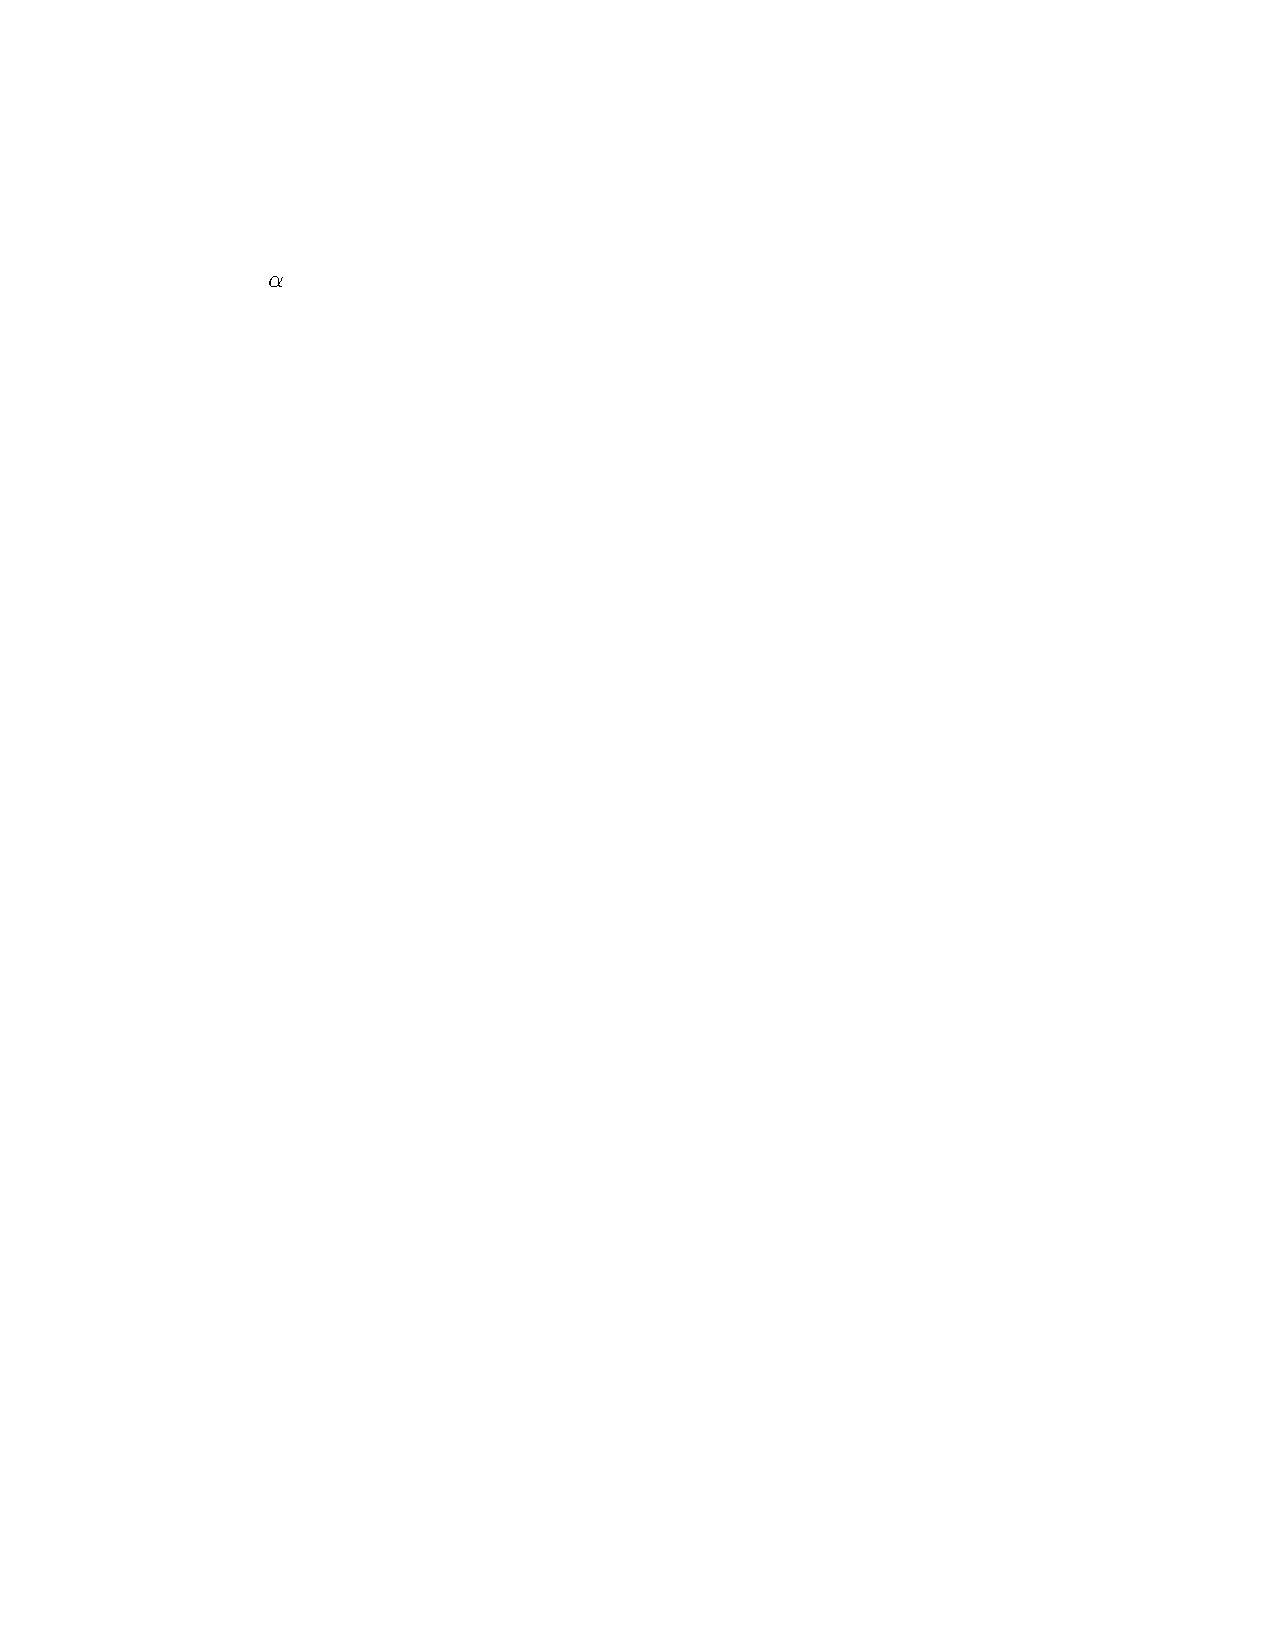
\includegraphics[width=0.6\linewidth]{a.pdf}
        \caption{Preprocessing steps}
        \label{fig:preprocessing_steps}
    \end{figure}

    \subsubsection*{Image augmentation}
    Image augmentation is a technique that is used to artificially increase the size of the dataset,
    in this case by slightly changing the images in the datasets. The main goal of the augmentation
    is to increase the image number, however another goal is to make the images more similar to the real
    images. First we start by noticing that the entire estimation problem of the heading error from
    a frontal image is symmetric with respect to the vertical axis. This means that we can just flip
    the image horizontally and invert the sign to the heading error to get a new valid sample for
    free. Aside from this symmetry, the data augmentation process can be summarized in the following
    steps:
    \begin{itemize}
        \item \textbf{Resize}: the images are resized to 4 times the final size to a 128x128
        square. The size is small for faster processing.
        \item \textbf{Random ellipses}: random ellipses are drawn on the image, with random
        positions and orientations and different shades of white. The idea behind this is to
        simulate strong light reflections, which are not present in the simulated environment. The
        ellipses also partially cover the image and can be considered a random erasing technique
        \citep*{random_erase}, which is a common data augmentation technique to reduce overfitting
        and increase robustness to occlusions. 
        \item \textbf{Dilation/erosion}: images are dilated or eroded (with a 20\% probability for
        each one) with a random kernel. This is done to simulate the effect of having wider or
        narrower lane markings. 
        \item \textbf{Preprocessing}: this is the preprocessing step, as described in the previous section.
        \item \textbf{Random shift}: the images are randomly shifted of a small amount of pixels
        across the vertical direction to account for possible camera misalignment. 
        \item \textbf{Noise}: the images are randomly corrupted with Gaussian noise, the variance
        of the noise is a hyperparameter that can be tuned. This is done to simulate the general
        robustness of the neural network to noise.
    \end{itemize}
    The augmentation steps are shown in Figure \ref{fig:augmentation_steps}.

    \begin{figure}
        \centering
        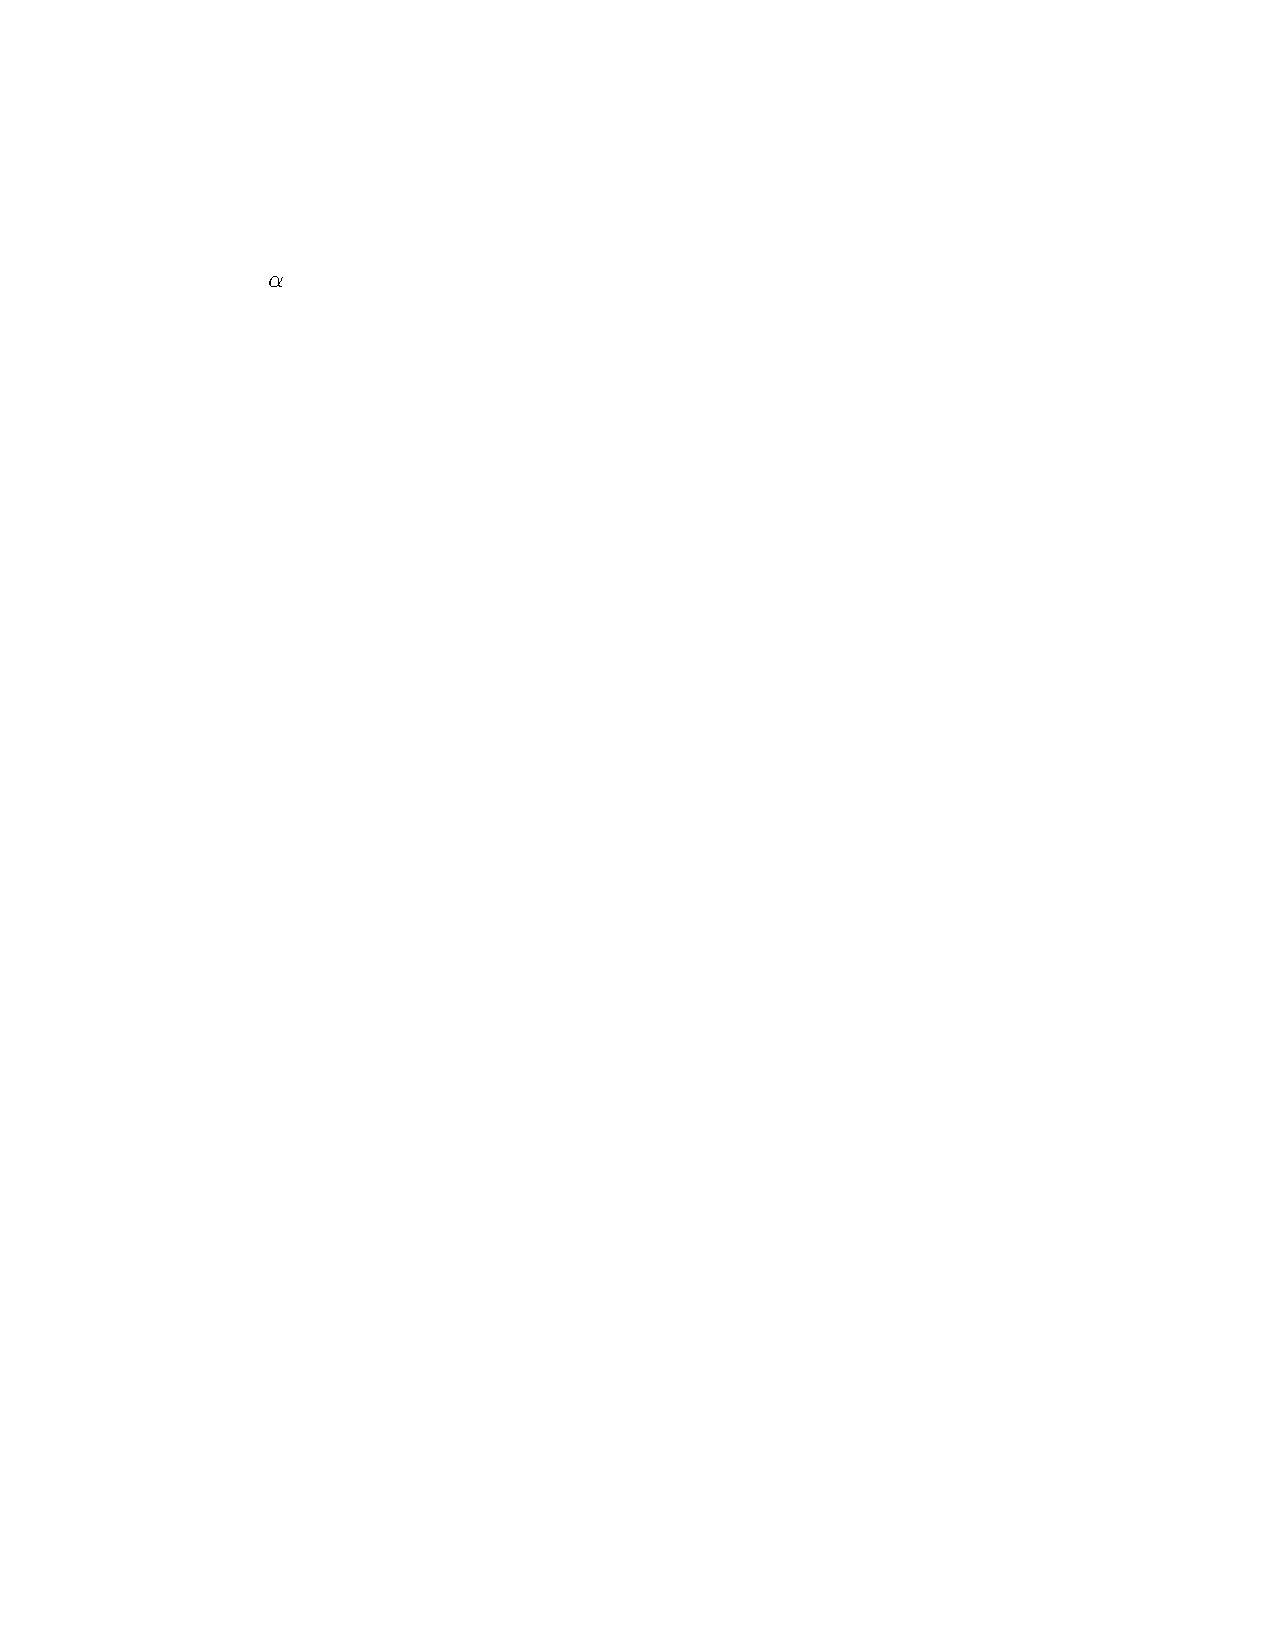
\includegraphics[width=0.6\linewidth]{a.pdf}
        \caption{Augmentation steps}
        \label{fig:augmentation_steps}
    \end{figure}

        
\subsection{Neural network training}
    In this section we will discuss the neural network architecture and the training process. When
    thinking about the design of the neural network one must take into account the fact that it will
    have to run on a real-time embedded system, and not a cluster of powerful GPUs. This means that 
    the neural network must be as small as possible, while still being able to perform well. Another
    important requirement is to being able to generalize well from the simulated data to the real data.

\subsubsection*{Network Architecture}
    In order to keep up with the performance required by the real-time constraints, the neural
    network has been designed with very few layers and very few parameters. The network architecture
    is inspired by the LeNet-5 \citep*{lecun} architecture, which is a very simple convolutional
    network that was originally designed for handwritten digit recognition. The design has been
    improved with the addition of batch normalization \citep*{batch_norm} and dropout
    \citep*{dropout}.
    The network is structured as a sequence of convolutional layers, followed by a sequence of fully
    connected layers; more specifically, the layers are the following:
    \begin{itemize}
        \item \textbf{1st 2D convolution}: 4 filters, with a kernel size of 5x5 and a stride of 1.
        It converts the original 32x32 image to 28x28.
        \item \textbf{ReLU}: activation function.
        \item \textbf{Dropout}: 30\% probability.
        \item \textbf{Pooling}: max pooling with a kernel size of 2x2 and a stride of 2. It converts
        the 28x28 image to 14x14.
        \item \textbf{Batch normalization}: normalization of the output of the previous layer.
        \item \textbf{2nd 2D convolution}: 16 filters, with a kernel size of 5x5 and a stride of 1.
        It converts the 14x14 image to 10x10.
        \item \textbf{ReLU}: activation function.
        \item \textbf{Dropout}: 30\% probability.
        \item \textbf{Pooling}: max pooling with a kernel size of 2x2 and a stride of 2. It converts
        the 10x10 image to 5x5.
        \item \textbf{Dropout}: 30\% probability.
        \item \textbf{3rd 2D convolution}: 32 filters, with a kernel size of 5x5 and a stride of 1.
        It converts the 5x5 image to 1x1.
        \item \textbf{ReLU}: activation function.
        \item \textbf{Flatten}: flattens the 1x1 image to a vector of 32 elements.
        \item \textbf{1st fully connected}: 16 neurons.
        \item \textbf{ReLU}: activation function.
        \item \textbf{2nd fully connected}: output layer, 1 neuron.
    \end{itemize}  

    The network takes as input a 32x32 grayscale image and outputs a single value representing the heading
    error. 

    The network architecture is shown in Figure \ref{fig:network_architecture}. The pytorch
    implementation can be found in the appendix.

    \begin{figure}
        \centering
        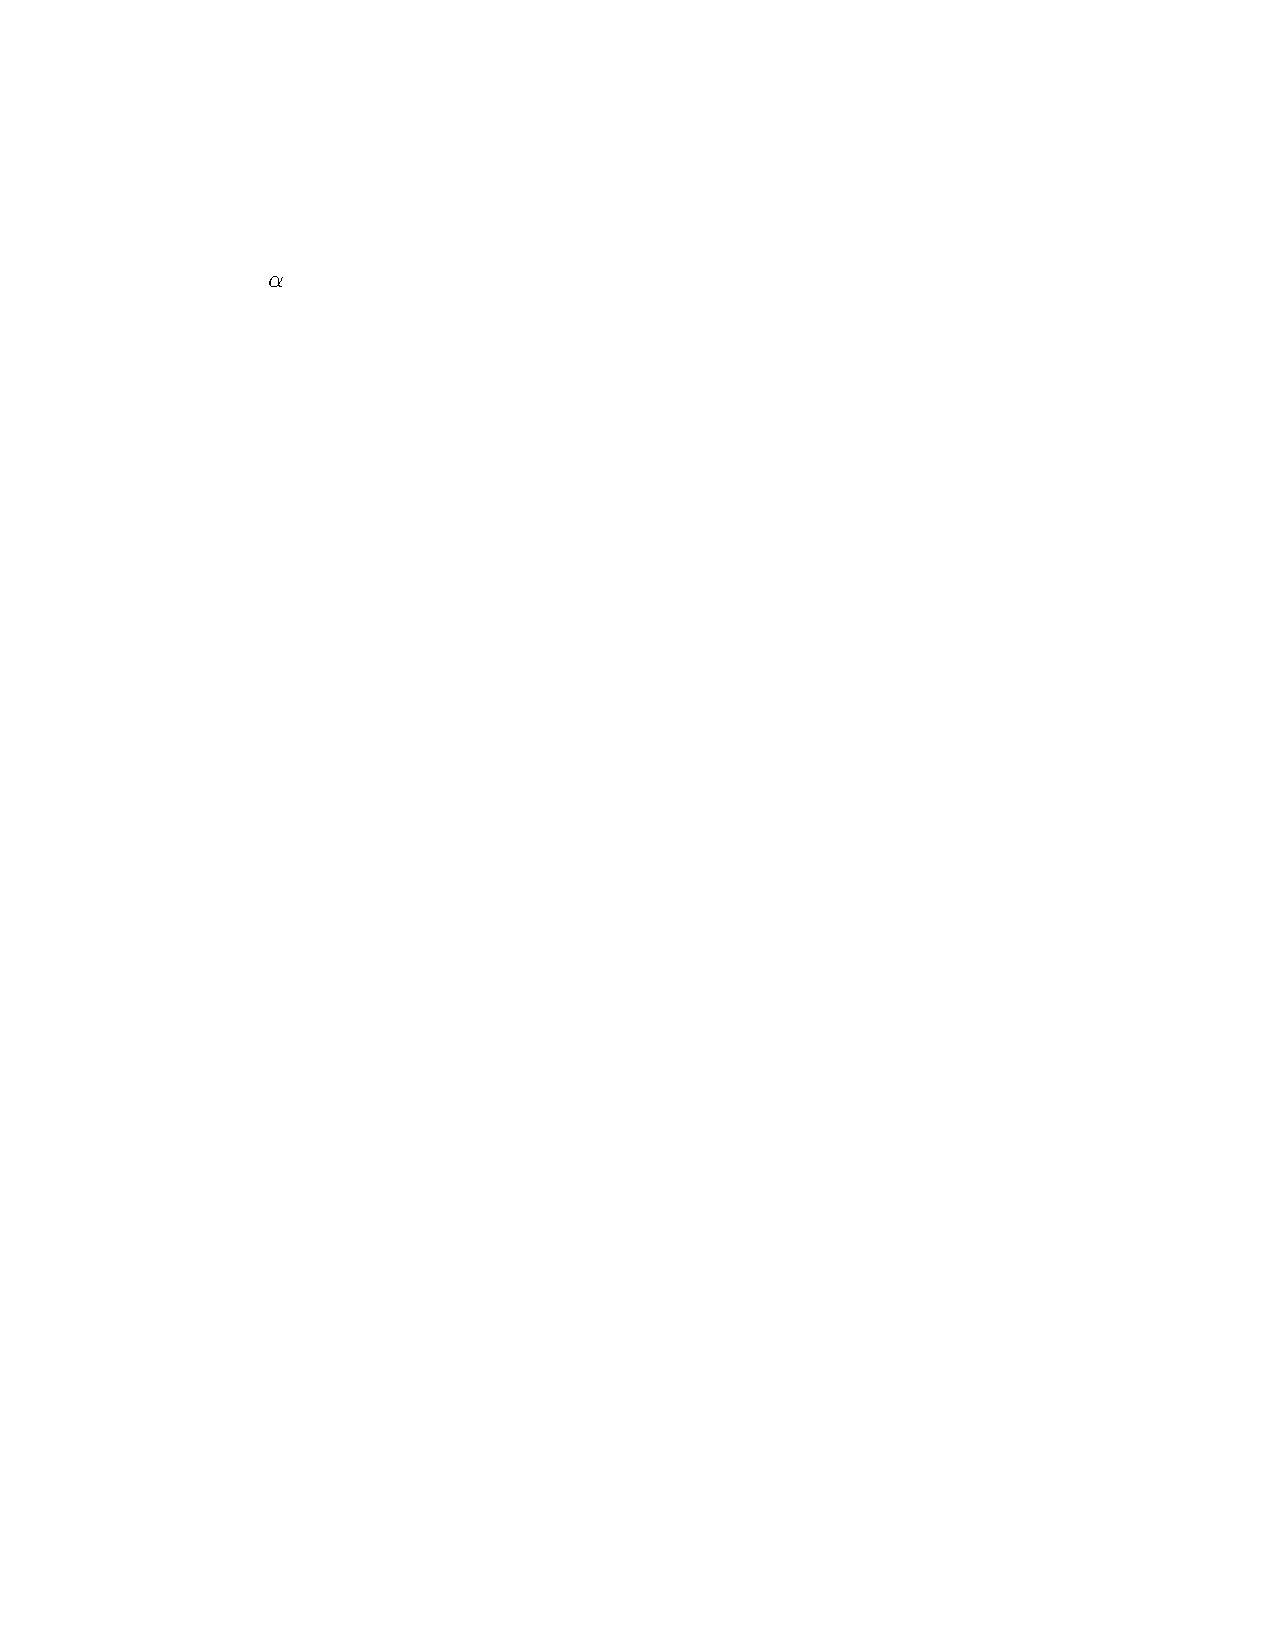
\includegraphics[width=0.6\linewidth]{a.pdf}
        \caption{Network architecture}
        \label{fig:network_architecture}
    \end{figure}

\subsubsection*{Training}
    keep practicing boy


% -Neural Network Estimation
    % -objectives of the network
    %     -estimating heading error
    %     -fast estimation
    %     -accuracy
    %     -continuity
    %     -(estimating the road)
    %     -explainability
    % -architecture
    %     -explain all the layers and what they do
    %         -layers, activations, weights initialization, biases initialization, and reasons for everything
    % -pytorch implementation
    % -Data flow
    %     -i/o of the network
    %         -image dimension
    %     -data preprocessing
    %     -data augmentation
    %         -explain how it works, reasons for doing it, and why it is necessary 
    %         -details of the augmentation, and possible variations
    %     -data normalization
    %     -data splitting
    %     -data loading
    %     -data batching
    %     -data shuffling
    % -training
    %     -optimizer
    %     -loss function
    %     -learning rate schedule
    %     -early stopping
    %     -validation
    %     -training loop
    %     -epochs
    %     -losses, and loss plots
    % -Network analysis
    %     -explanation of standard network analysis methods
    %     -visualizations of conv filters
    %     -visualizations of fully connected layers
    %     -layer activations
    %     -layer weights
    %     -layer biases
    % -(Extensions)
    %     -(multiple frames)
    %     -(time coherence)
    %     -(continuity)
    %     -(multiple points estimation, path ahead)
    %     -variable speed
    %     -state estimation
        % -reducing dataset size

\subsection{Online estimation}
    Talk about the online estimationq

\section{Results} \label{sec:results}

\subsection{Experimental setup} \label{sec:exp_setup}
-Experimental setup
    % -explanation of the experimental setup in the sparcs lab, Vicon system etc..
    % -explanation of data collection methodologies
    % -analysis of performance wrt different parameters combinations and values, graphs tables etc..
    %     Parameters:
    %     -noise levels in training path
    %         -steering noise, quantified by variance of distance car-path; diff yaw car-yaw path
    %         -speed noise, quantified by variance of speed value from the desired mean speed
    %     -image dimension, images are downsized to achieve faster computation, evaluate the impact
    %     -network architecture variations:
    %         -num conv layers
    %         -num fully connected layers
    %         -num hidden units in each layer
    %         -complexity metric of network (?search papers)
    %     -fps of the video
    %     -length of the training dataset
    %         -length of the video
    %         -car speed
    %         -length of the simulation path
    %         -simulation time 
    %     -training Parameters    
    %         -learning rate
    %         -batch size
    %         -optimizer
    %         -epochs
    %     -image augmentation
    %         -noise level
    %         -

\subsection{Datasets analysis}
Talk about the datasets, the possible variations, lots of images

\subsection{Network analysis}
Talk about the network, lots of images

\subsection{Analysis of hyperparameters}
    Talk about the big hyperparameters study and how it has been implemented

\subsection{Numerical results}
    Talk about the results, the graphs, the tables, the numbers, the analysis

\section{Control loop application}
    Talk about the control loop, the implementation, the results, the analysis

% -aggiungere il control loop

% -ENFATIZZARE L'ASSENZA DI RITARDO NELLA NN



\newpage
\section{Conclusion and Future Work}
end




\newpage
\section{Appendix}
consider adding full derivation of the bicycle model \url{https://www.youtube.com/watch?v=HqNdBiej23I&ab_channel=Prof.GeorgSchildbach%2CUniversityofLuebeck}
\url{https://thomasfermi.github.io/Algorithms-for-Automated-Driving/Control/BicycleModel.html}
\url{http://code.eng.buffalo.edu/dat/sites/model/bicycle.html#:~:text=motion%20under%20the%20assumption%20of,hard%20braking%20and%20steering%20maneuvers.}
\url{https://ieeexplore.ieee.org/document/9311987}

\subsection{Python implementation of heading error calculation}
add the python version of the previously described algorithm.

consider adding derivation of the pure pursuit
\url{https://ieeexplore.ieee.org/document/9368694}


\newpage

% references %note: delete the .bib file every time uadd a reference
\begin{filecontents}{References.bib}
    %vehicle model
    @article{doi:10.1080/00423119508969086,
        author = { Dirk E.   Smith  and  John M. Starkey},
        title = {Effects of Model Complexity on the Performance of Automated Vehicle Steering Controllers: Model Development, Validation and Comparison},
        journal = {Vehicle System Dynamics},
        volume = {24},
        number = {2},
        pages = {163-181},
        year  = {1995},
        publisher = {Taylor & Francis},
        doi = {10.1080/00423119508969086},
        URL = {https://doi.org/10.1080/00423119508969086},
        eprint = { https://doi.org/10.1080/00423119508969086}
    }
    @INPROCEEDINGS{7995816,
        author={Polack, Philip and Altché, Florent and d'Andréa-Novel, Brigitte and de La Fortelle, Arnaud},
        booktitle={2017 IEEE Intelligent Vehicles Symposium (IV)}, 
        title={The kinematic bicycle model: A consistent model for planning feasible trajectories for autonomous vehicles?}, 
        year={2017},
        volume={},
        number={},
        pages={812-818},
        doi={10.1109/IVS.2017.7995816}
    }
    @INPROCEEDINGS{9368694,
        author={Huang, Yaofu and Tian, Zengshan and Jiang, Qing and Xu, Junxing},
        booktitle={2020 IEEE 2nd International Conference on Civil Aviation Safety and Information Technology (ICCASIT}, 
        title={Path Tracking Based on Improved Pure Pursuit Model and PID}, 
        year={2020},
        volume={},
        number={},
        pages={359-364},
        doi={10.1109/ICCASIT50869.2020.9368694}
    }
    %ros
    @inproceedings{quigley2009ros,
        title={ROS: an open-source Robot Operating System},
        author={Quigley, Morgan and Conley, Ken and Gerkey, Brian and Faust, Josh and Foote, Tully and Leibs, Jeremy and Wheeler, Rob and Ng, Andrew Y and others},
        booktitle={ICRA workshop on open source software},
        volume={3},
        number={3.2},
        pages={5},
        year={2009},
        organization={Kobe, Japan}
    }
    %gazebo simulator
    @INPROCEEDINGS{1389727,
        author={Koenig, N. and Howard, A.},
        booktitle={2004 IEEE/RSJ International Conference on Intelligent Robots and Systems (IROS) (IEEE Cat. No.04CH37566)}, 
        title={Design and use paradigms for Gazebo, an open-source multi-robot simulator}, 
        year={2004},
        volume={3},
        number={},
        pages={2149-2154 vol.3},
        doi={10.1109/IROS.2004.1389727}
    }
    %carla sim
    @inproceedings{dosovitskiy2017carla,
        title={CARLA: An open urban driving simulator},
        author={Dosovitskiy, Alexey and Ros, German and Codevilla, Felipe and Lopez, Antonio and Koltun, Vladlen},
        booktitle={Conference on robot learning},
        pages={1--16},
        year={2017},
        organization={PMLR}
    }
    %pure pursuit
    @techreport{coulter1992implementation,
        title={Implementation of the pure pursuit path tracking algorithm},
        author={Coulter, R Craig},
        year={1992},
        institution={Carnegie-Mellon UNIV Pittsburgh PA Robotics INST}
    }
    @INPROCEEDINGS{7796574,
        author={Ohta, Hiroki and Akai, Naoki and Takeuchi, Eijiro and Kato, Shinpei and Edahiro, Masato},
        booktitle={2016 IEEE 4th International Conference on Cyber-Physical Systems, Networks, and Applications (CPSNA)}, 
        title={Pure Pursuit Revisited: Field Testing of Autonomous Vehicles in Urban Areas}, 
        year={2016},
        volume={},
        number={},
        pages={7-12},
        doi={10.1109/CPSNA.2016.10}
    }
    %clothoid 1
    @ARTICLE{6646277,
        author={Brezak, Mišel and Petrović, Ivan},
        journal={IEEE Transactions on Robotics}, 
        title={Real-time Approximation of Clothoids With Bounded Error for Path Planning Applications}, 
        year={2014},
        volume={30},
        number={2},
        pages={507-515},
        doi={10.1109/TRO.2013.2283928}
    }
    %ref in clothoid 1
    @inproceedings{kanayama1988smooth,
        title={Smooth Local Path Planning for Autonomous Vehicles (Part II. Cubic Spirals)},
        author={Kanayama, Y and Hartman, B},
        booktitle={Proc. Annual Conference of Robotics Society of Japan},
        pages={93--96},
        year={1988}
        }
        @article{delingette1991trajectory, 
        title={Trajectory generation with curvature constraint based on energy minimization},
        author={Delingette, Herv{\'e} and Hebert, Martial and Ikeuchi, Katsushi},
        year={1991},
        publisher={Carnegie Mellon University}
    }
    @inproceedings{segovia1991comparative,
        title={Comparative study of the different methods of path generation for a mobile robot in a free environment},
        author={Segovia, A and Rombaut, M and Preciado, A and Meizel, D},
        booktitle={Fifth International Conference on Advanced Robotics' Robots in Unstructured Environments},
        pages={1667--1670},
        year={1991},
        organization={IEEE}
    }
    @inproceedings{lau2009kinodynamic,
        title={Kinodynamic motion planning for mobile robots using splines},
        author={Lau, Boris and Sprunk, Christoph and Burgard, Wolfram},
        booktitle={2009 IEEE/RSJ International Conference on Intelligent Robots and Systems},
        pages={2427--2433},
        year={2009},
        organization={IEEE}
    }
    @article{shanmugavel2010co,
        title={Co-operative path planning of multiple UAVs using Dubins paths with clothoid arcs},
        author={Shanmugavel, Madhavan and Tsourdos, Antonios and White, Brian and {\.Z}bikowski, Rafa{\l}},
        journal={Control engineering practice},
        volume={18},
        number={9},
        pages={1084--1092},
        year={2010},
        publisher={Elsevier}
    }
    @ARTICLE{388788,
        author={Fleury, S. and Soueres, P. and Laumond, J.-P. and Chatila, R.},
        journal={IEEE Transactions on Robotics and Automation}, 
        title={Primitives for smoothing mobile robot trajectories}, 
        year={1995},
        volume={11},
        number={3},
        pages={441-448},
        doi={10.1109/70.388788}
    }
    @article{BOISSONNAT1999613,
        title = {Shortest plane paths with bounded derivative of the curvature},
        journal = {Comptes Rendus de l'Académie des Sciences - Series I - Mathematics},
        volume = {329},
        number = {7},
        pages = {613-618},
        year = {1999},
        issn = {0764-4442},
        doi = {https://doi.org/10.1016/S0764-4442(00)80011-7},
        url = {https://www.sciencedirect.com/science/article/pii/S0764444200800117},
        author = {Jean-Daniel Boissonnat and André Cérézo and Elena V. Degtiariova-Kostova and Vladimir P. Kostov and Juliette Leblond},
    }
    @ARTICLE{1362698,
        author={Fraichard, T. and Scheuer, A.},
        journal={IEEE Transactions on Robotics}, 
        title={From Reeds and Shepp's to continuous-curvature paths}, 
        year={2004},
        volume={20},
        number={6},
        pages={1025-1035},
        doi={10.1109/TRO.2004.833789}
    }
    @phdthesis{meidenbauer2007investigation,
        title={An investigation of the clothoid steering model for autonomous vehicles},
        author={Meidenbauer, Kennneth Richard},
        year={2007},
        school={Virginia Tech}
    }
    @article{urmson2008autonomous,
        title={Autonomous driving in urban environments: Boss and the urban challenge},
        author={Urmson, Chris and Anhalt, Joshua and Bagnell, Drew and Baker, Christopher and Bittner, Robert and Clark, MN and Dolan, John and Duggins, Dave and Galatali, Tugrul and Geyer, Chris and others},
        journal={Journal of field Robotics},
        volume={25},
        number={8},
        pages={425--466},
        year={2008},
        publisher={Wiley Online Library}
    }
    % clothoid 2
    @INPROCEEDINGS{7942658,
        author={Atmosudiro, Agus and Verl, Alexander and Lechler, Armin and Schwarz, Gerwin},
        booktitle={2017 3rd International Conference on Control, Automation and Robotics (ICCAR)}, 
        title={A Clothoid based real-time interpolation concept for path smoothing}, 
        year={2017},
        volume={},
        number={},
        pages={41-46},
        doi={10.1109/ICCAR.2017.7942658}
    }
    @ARTICLE{7962257,
        author={Chen, Yong and Cai, Yiyu and Zheng, Jianmin and Thalmann, Daniel},
        journal={IEEE Transactions on Robotics}, 
        title={Accurate and Efficient Approximation of Clothoids Using Bézier Curves for Path Planning}, 
        year={2017},
        volume={33},
        number={5},
        pages={1242-1247},
        doi={10.1109/TRO.2017.2699670}
    }
    @article{nutbourne1972curvature,
        title={Curvature profiles for plane curves},
        author={Nutbourne, AW and McLellan, PM and Kensit, RML},
        journal={Computer-aided design},
        volume={4},
        number={4},
        pages={176--184},
        year={1972},
        publisher={Elsevier}
    }
    % frenel integrals
    @ARTICLE{41470,
        author={Barsky, B.A. and DeRose, T.D.},
        journal={IEEE Computer Graphics and Applications}, 
        title={Geometric continuity of parametric curves: three equivalent characterizations}, 
        year={1989},
        volume={9},
        number={6},
        pages={60-69},
        doi={10.1109/38.41470}
    }
    %clothoid approximation 6646277,7962257,4543548
    @INPROCEEDINGS{4543548,
        author={Montes, Nicolas and Herraez, Alvaro and Armesto, Leopoldo and Tornero, Josep},
        booktitle={2008 IEEE International Conference on Robotics and Automation}, 
        title={Real-time clothoid approximation by Rational Bezier curves}, 
        year={2008},
        volume={},
        number={},
        pages={2246-2251},
        doi={10.1109/ROBOT.2008.4543548}
    }
    %pyclothoids library and Bertolazzi papers: https://doi.org/10.1002/mma.3114, BERTOLAZZI201899,
    %https://doi.org/10.1002/mma.4700, doi:10.1137/18M1200439
    @misc{pyclothoids,
        author = {Schmitz, Johannes and phillipd94},
        title = {{pyclothoids}},
        howpublished = "\url{https://github.com/phillipd94/pyclothoids}",
        year = {2020}, 
        note = "[Online; accessed 2022]"
    }
    @article{https://doi.org/10.1002/mma.3114,
        author = {Bertolazzi, Enrico and Frego, Marco},
        title = {G1 fitting with clothoids},
        journal = {Mathematical Methods in the Applied Sciences},
        volume = {38},
        number = {5},
        pages = {881-897},
        keywords = {clothoid, Fresnel integrals, Hermite G1 interpolation},
        doi = {https://doi.org/10.1002/mma.3114},
        url = {https://onlinelibrary.wiley.com/doi/abs/10.1002/mma.3114},
        eprint = {https://onlinelibrary.wiley.com/doi/pdf/10.1002/mma.3114},
        year = {2015}
    }
    @article{BERTOLAZZI201899,
        title = {On the G2 Hermite Interpolation Problem with clothoids},
        journal = {Journal of Computational and Applied Mathematics},
        volume = {341},
        pages = {99-116},
        year = {2018},
        issn = {0377-0427},
        doi = {https://doi.org/10.1016/j.cam.2018.03.029},
        url = {https://www.sciencedirect.com/science/article/pii/S0377042718301924},
        author = {Enrico Bertolazzi and Marco Frego},
        keywords = {Clothoid, Euler spiral, Cornu spiral, 
                        interpolation, Fitting},
    }
    @article{https://doi.org/10.1002/mma.4700,
        author = {Bertolazzi, Enrico and Frego, Marco},
        title = {Interpolating clothoid splines with curvature continuity},
        journal = {Mathematical Methods in the Applied Sciences},
        volume = {41},
        number = {4},
        pages = {1723-1737},
        keywords = {clothoid, fresnel integrals, splines},
        doi = {https://doi.org/10.1002/mma.4700},
        url = {https://onlinelibrary.wiley.com/doi/abs/10.1002/mma.4700},
        eprint = {https://onlinelibrary.wiley.com/doi/pdf/10.1002/mma.4700},
        year = {2018}
    }
    @article{doi:10.1137/18M1200439,
        author = {Frego, Marco and Bertolazzi, Enrico},
        title = {Point-Clothoid Distance and Projection Computation},
        journal = {SIAM Journal on Scientific Computing},
        volume = {41},
        number = {5},
        pages = {A3326-A3353},
        year = {2019},
        doi = {10.1137/18M1200439},
        URL = {https://doi.org/10.1137/18M1200439},
        eprint = {https://doi.org/10.1137/18M1200439}
    }
    %Dijkstra algoritmm
    @article{dijkstra1959note,
        title={A note on two problems in connexion with graphs},
        author={Dijkstra, Edsger W},
        journal={Numerische mathematik},
        volume={1},
        number={1},
        pages={269--271},
        year={1959},
        publisher={Springer}
    }

    %performance metrics
    @INPROCEEDINGS{6977166,
        author={Satzoda, Ravi Kumar and Trivedi, Mohan M.},
        booktitle={2014 22nd International Conference on Pattern Recognition}, 
        title={On Performance Evaluation Metrics for Lane Estimation}, 
        year={2014},
        volume={},
        number={},
        pages={2625-2630},
        doi={10.1109/ICPR.2014.453}
    }
    @ARTICLE{1603550,
        author={McCall, J.C. and Trivedi, M.M.},
        journal={IEEE Transactions on Intelligent Transportation Systems}, 
        title={Video-based lane estimation and tracking for driver assistance: survey, system, and evaluation}, 
        year={2006},
        volume={7},
        number={1},
        pages={20-37},
        doi={10.1109/TITS.2006.869595}
    }
    @article{cheng2007lane,
        title={Lane tracking with omnidirectional cameras: Algorithms and evaluation},
        author={Cheng, Shinko Yuanhsien and Trivedi, Mohan Manubhai},
        journal={EURASIP Journal on Embedded Systems},
        volume={2007},
        pages={1--8},
        year={2007},
        publisher={Springer}
    }
    @INPROCEEDINGS{6728507,
        author={Satzoda, R. K. and Trivedi, Mohan M.},
        booktitle={16th International IEEE Conference on Intelligent Transportation Systems (ITSC 2013)}, 
        title={Selective salient feature based lane analysis}, 
        year={2013},
        volume={},
        number={},
        pages={1906-1911},
        doi={10.1109/ITSC.2013.6728507}}
    @ARTICLE{9398517,
        author={Zhang, Youcheng and Lu, Zongqing and Zhang, Xuechen and Xue, Jing-Hao and Liao, Qingmin},
        journal={IEEE Transactions on Intelligent Transportation Systems}, 
        title={Deep Learning in Lane Marking Detection: A Survey}, 
        year={2022},
        volume={23},
        number={7},
        pages={5976-5992},
        doi={10.1109/TITS.2021.3070111}}

    %CANNY
    @article{canny,
        author = {Canny, John},
        year = {1986},
        month = {12},
        pages = {679 - 698},
        title = {A Computational Approach To Edge Detection},
        volume = {PAMI-8},
        isbn = {9780080515816},
        journal = {Pattern Analysis and Machine Intelligence, IEEE Transactions on},
        doi = {10.1109/TPAMI.1986.4767851}
        }
    @misc{random_erase,
        doi = {10.48550/ARXIV.1708.04896},
        url = {https://arxiv.org/abs/1708.04896},
        author = {Zhong, Zhun and Zheng, Liang and Kang, Guoliang and Li, Shaozi and Yang, Yi},
        keywords = {Computer Vision and Pattern Recognition (cs.CV), FOS: Computer and information sciences, FOS: Computer and information sciences},
        title = {Random Erasing Data Augmentation},
        publisher = {arXiv},
        year = {2017},
        copyright = {arXiv.org perpetual, non-exclusive license}
        }
    %lecun
    @article{lecun,
        author = {Lecun, Yann and Haffner, Patrick and Bengio, Y.},
        year = {2000},
        month = {08},
        pages = {},
        title = {Object Recognition with Gradient-Based Learning}
        }
    @misc{batch_norm,
        doi = {10.48550/ARXIV.1502.03167},
        url = {https://arxiv.org/abs/1502.03167},
        author = {Ioffe, Sergey and Szegedy, Christian},
        keywords = {Machine Learning (cs.LG), FOS: Computer and information sciences, FOS: Computer and information sciences},
        title = {Batch Normalization: Accelerating Deep Network Training by Reducing Internal Covariate Shift},
        publisher = {arXiv},
        year = {2015},
        copyright = {arXiv.org perpetual, non-exclusive license}
      }
    @article{dropout,
      author  = {Nitish Srivastava and Geoffrey Hinton and Alex Krizhevsky and Ilya Sutskever and Ruslan Salakhutdinov},
      title   = {Dropout: A Simple Way to Prevent Neural Networks from Overfitting},
      journal = {Journal of Machine Learning Research},
      year    = {2014},
      volume  = {15},
      number  = {56},
      pages   = {1929--1958},
      url     = {http://jmlr.org/papers/v15/srivastava14a.html}
    }
      



\end{filecontents}

\bibliographystyle{unsrt}
\bibliography{References}



\newpage









\end{document}